\documentclass[10pt]{article}
\usepackage{titling}
\usepackage{blindtext}
\usepackage {amssymb,latexsym}
\usepackage {amsmath}
\usepackage{graphicx}
\usepackage{comment}
\usepackage{amsthm}
\usepackage{relsize}
\usepackage[margin=1in]{geometry}
\usepackage[latin1]{inputenc}
\usepackage{fancyhdr}
\usepackage{pgfplots}
\pgfplotsset{compat=1.14}
\usepackage{amscd}
\usepackage{hyperref}
\usepackage{graphicx}
\usepackage{relsize}
\usepackage{newlfont}
\usepackage{amssymb}
\usepackage{youngtab}
\usepackage{young}
\usepackage{stmaryrd} 
\usepackage{mathtools}
\usepackage{tikz}
\usetikzlibrary{shapes, backgrounds} 
\usepackage{tikz-cd}
\usepackage{amsthm}
\usepackage{authblk} %address in front page
\usepackage{enumerate,enumitem}
\usepackage{mathrsfs}
\usepackage{soul} %strike out
\usepackage[scr=rsfs,cal=boondox]{mathalfa} 
\newenvironment {innerproof}{\small {\sc Proof:}}{{\hspace*{\fill}
$\bigtriangledown$}}
\newtheorem {lemma} {Lemma}
\newtheorem {proposition} [lemma] {Proposition}
\newtheorem {theorem} [lemma] {Theorem}
\newtheorem {corollary} [lemma] {Corollary}
\newtheorem {definition}[lemma] {Definition}
\theoremstyle{definition}
\newtheorem{remark}[lemma]{Remark}
\newtheorem{example}[lemma]{Example}
\newenvironment{invisible}{{\noindent\sc \colorbox{yellow}{Invisible:}\;}\color{gray}}{\medskip}
\excludecomment{invisible}
%%%%MACROS%%%%%
\newcommand{\g}{\mathfrak{g}}
\newcommand{\wt}{\vartriangleright}
\newcommand{\bt}{\blacktriangleright}
\renewcommand{\r}{\mathfrak{r}}
\newcommand{\s}{\mathfrak{s}}
\renewcommand{\l}{\mathfrak{l}}
\newcommand{\n}{\mathfrak{n}}
\newcommand{\R}{\mathfrak{R}}
\renewcommand{\L}{\mathfrak{L}}
\newcommand{\Der}{\mathrm{Der}}
\newcommand{\Aut}{\mathrm{Aut}}
\newcommand{\ad}{\mathrm{ad}}
\newcommand{\ten}{\otimes}
\renewcommand{\wp}{\diamond}
\newcommand{\ot}{\otimes}
\newcommand{\ab}[2]{\langle #1,#2\rangle}
\newcommand{\abd}[2]{\langle #1,#2\rangle^{\bullet}}
%%%%%%%%%%%%%%%%%%%%%%%%
\DeclareFontFamily{U}{mathb}{}
\DeclareFontShape{U}{mathb}{m}{n}{<-5.5> mathb5 <5.5-6.5> mathb6 
<6.5-7.5> mathb7 <7.5-8.5> mathb8 <8.5-9.5> mathb9 <9.5-11> mathb10 
<11-> mathb12}{}
\DeclareSymbolFont{mathb}{U}{mathb}{m}{n}
\DeclareFontSubstitution{U}{mathb}{m}{n}
\DeclareMathSymbol{\bp}{\mathbin}{mathb}{"0C}
%%%%%%%%%%%%%%%%%%%%%%%%%

\makeatletter
\@addtoreset{equation}{section}
\def\theequation{\thesection.\arabic{equation}}
\makeatother


\begin{document}
\setlength{\parindent}{0pt} % no indentation
\title {\textbf{An infinitesimal deformation of the post-Lie and post-Hopf algebra correspondence}}

\author[a]{Andrea Rivezzi}
\author[b]{Andrea Sciandra}
\author[a]{Thomas Weber}

\affil[a]{{\sl
{Mathematical Institute of Charles University}}

{\sl Sokolovsk\'a 49/83, 186 75 Prague 8, Czech Republic}

{~}}

\affil[b]{{\sl
{D\'epartement de Math\'ematiques, Universit\'e Libre de Bruxelles}}
	
{\sl Boulevard du Triomphe, B-1050 Bruxelles, Belgium}  }
  
%\begin{titlingpage}


%\thispagestyle{empty}
\date{}
\maketitle
\vspace{-1cm}
\begin{abstract}
\noindent
We describe infinitesimal deformations of post-Lie algebras and post-Hopf algebras and prove that the adjunction given by the universal enveloping algebra and primitive elements functors is compatible with the infinitesimal structure. When restricted to connected and cocommutative infinitesimal post-Hopf algebras, this becomes an equivalence of categories, which constitutes an extension of the Cartier--Milnor--Moore theorem. 
We classify infinitesimal post-Lie structures on $\mathfrak{sl}(2)$, and discuss a class of infinitesimal post-Lie algebras emerging from flat connections with covariantly-constant torsion. Moreover, we classify infinitesimal post-Hopf structures on Sweedler's Hopf algebra. Cocommutative infinitesimal post-Hopf algebras induce a Hochschild 2-cocycle on the associated subadjacent Hopf algebra. Finally, we prove that the quadratic operad of infinitesimal post-Lie algebras is Koszul, by using a filtered distributive law between the operads of Lie algebras and bi-magmas.
\end{abstract}
2020 Mathematics Subject Classification: 17B05, 16T05, 16S30, 18M70. \\ 
Keywords: (Infinitesimal) post-Lie algebras, (Infinitesimal) post-Hopf algebras, Operads.


\tableofcontents


\section*{Introduction}
Post-Lie algebras have been introduced by B. Vallette in \cite{Vallette} in an operadic context as the Koszul dual of commutative trialgebras. Since then, post-Lie algebras have gained broad recognition since they also appear in geometric frameworks, such as the numerical integration of manifolds \cite{CE-FM-K} and in the presence of flat connections on smooth manifolds with covariantly-constant torsion \cite{ML}, but also in the renormalization of stochastic partial differential equations \cite{BST}. Algebraically, a \emph{post-Lie algebra} is a Lie algebra $(\mathfrak{g},[\cdot,\cdot])$ endowed with an additional bilinear operation $\wt\colon\mathfrak{g}\times\mathfrak{g}\to\mathfrak{g}$ such that its restriction to the first component is a derivation, satisfying
$$
[x,y] \wt z = x \wt (y \wt z) - y \wt (x \wt z) - (x \wt y) \wt z + (y \wt x) \wt z
$$
for all $x,y,z\in\mathfrak{g}$. The right-hand side of the above axiom constitutes a pre-Lie algebra condition, and thus post-Lie algebras with trivial Lie bracket recover pre-Lie algebras. Moreover, from an arbitrary post-Lie algebra $(\mathfrak{g},[\cdot,\cdot],\wt)$ one constructs another Lie algebra structure
	\begin{equation}
		[\cdot,\cdot]_{\wt}:=[\cdot,\cdot]+\wt-\wt^\mathrm{op}
	\end{equation}
on the vector space $\mathfrak{g}$, the so-called \emph{subadjacent Lie algebra}, where $\wt^\mathrm{op}$ denotes the precomposition of $\wt$ with the flip. For $[\cdot,\cdot]=0$ this is the well-known Lie bracket of a pre-Lie algebra.

On the universal enveloping algebra $\mathrm{U}(\mathfrak{g})$ of a post-Lie algebra $(\mathfrak{g},[\cdot,\cdot]\wt)$, one constructs a coalgebra map $\wp\colon\mathrm{U}(\mathfrak{g})\otimes\mathrm{U}(\mathfrak{g})\to\mathrm{U}(\mathfrak{g})$ by suitably extending the map $\wt$, which structures $\mathrm{U}(\mathfrak{g})$ as a cocommutative \emph{post-Hopf algebra}. The notion of post-Hopf algebra has been introduced in \cite{LST} for (not necessarily cocommutative) Hopf algebras $H$ with coalgebra maps $\wp\colon H\otimes H\to H$ satisfying appropriate axioms (see Definition \ref{def:PH}). From a \textit{cocommutative} post-Hopf algebra $(H,\wp)$ one constructs a Hopf algebra $H_{\wp}$, the \emph{subadjacent Hopf algebra}, which coincides with $H$ as a coalgebra, but which is endowed with a $\wp$-``twisted'' product $\star_\wp$ and antipode $S_\wp$. The subadjacent Hopf algebra is compatible with the subadjacent Lie algebra, in the sense that the diagram
	\begin{equation*}
	\begin{tikzcd}
		(\mathfrak{g},[\cdot,\cdot],\wt) \arrow[rr, maps to, "\mathrm{U}"] \arrow[d, maps to, swap, "\text{subadjacent}"] & & (\mathrm{U}(\mathfrak{g}),\wp) \arrow[d, maps to, "\text{subadjacent}"]\\
		\mathfrak{g}_{\wt}:=(\mathfrak{g},[\cdot,\cdot]_{\wt}) \arrow[rr, maps to, "\mathrm{U}"] & & \mathrm{U}(\mathfrak{g}_{\wt})\cong\mathrm{U}(\mathfrak{g})_{\wp}
	\end{tikzcd}
	\end{equation*}
	commutes, see again \cite{LST}. The assumption of cocommutativity is also crucial in the realm of the \textit{quantum Yang--Baxter equation} (QYBE). In fact, given a cocommutative post-Hopf algebra $(H,\wp)$, the following linear map is a solution to the braid equation $\sigma_{12}\sigma_{23}\sigma_{12}=\sigma_{23}\sigma_{12}\sigma_{23}$ on the vector space $H$:
\begin{equation}
\sigma(a\ot b):=(a_{1}\wp b_{1})\ot(S_{\wp}(a_{2}\wp b_{2})\star_{\wp}a_{3}\star_{\wp}b_{3}),\qquad \text{for all}\ a,b\in H.
\end{equation}
Equivalently, $\tau\sigma$ satisfies the QYBE, with $\tau$ the flip map of vector spaces. In the cocommutative setting, post-Hopf algebras are in fact equivalent to Hopf braces introduced in \cite{AGV} and to matched pairs of actions on (cocommutative) Hopf algebras. 

Conversely, the subspace of primitive elements $\mathrm{P}(H)$ of a post-Hopf algebra $H$ becomes a post-Lie algebra when endowed with the commutator. The universal enveloping algebra and primitives determine an adjoint pair of functors 
\begin{equation}\label{adj:LieHopf}
	\begin{tikzcd}
		\mathrm{PLie} \arrow[rr, bend left, "\mathrm{U}"] & \perp & \mathrm{PHopf} \arrow[ll, bend left, "P"]
	\end{tikzcd}
	\end{equation}
	for the categories $\mathrm{PLie}$ of post-Lie algebras and $\mathrm{PHopf}$ of post-Hopf algebras. If the base field has characteristic 0, a \emph{Cartier--Milnor--Moore theorem} \cite{MilnorMoore} can be established for cocommutative, connected post-Hopf algebras \cite{Catoire,ZD}, namely, the above adjunction becomes an equivalence of categories when replacing $\mathrm{PHopf}$ with this subcategory. Note that, being isomorphic to the category of cocommutative Hopf braces, by the results proven in \cite{GS}, the category of cocommutative post-Hopf algebras is semi-abelian \cite{Semiabelian} and equipped with a \textit{torsion theory} in the sense of \cite{BournGran}, whose torsion subcategory is given by universal enveloping algebras of post-Lie algebras and torsion-free subcategory is given by group algebras over post-groups \cite{BGST}, that are equivalent to skew braces \cite{GuVe}. In particular, for any cocommutative post-Hopf algebra, a short exact sequence can be determined, where the torsion and torsion-free objects belong to the aforementioned categories.
\medskip

\noindent
For these reasons, it is justified to expect additional algebraic structure on a post-Lie algebra to correspond to additional structure on the post-Hopf algebra level and vice versa. We focus on this correspondence and discuss infinitesimal deformations, leading to the notions of \emph{infinitesimal} post-Lie and post-Hopf algebras. We define infinitesimal post-Lie algebras and infinitesimal post-Hopf algebras as post-Lie algebras $(\mathfrak{g},[\cdot,\cdot],\wt)$ and post-Hopf algebras $(H,\wp)$ together with (bi)linear maps $\bt\colon\mathfrak{g}\times\mathfrak{g}\to\mathfrak{g}$ and $\bp\colon H\otimes H\to H$ subject to axioms (see Definitions \ref{def:infinitesimalPostLie} and \ref{def:infinitesimalpostHopf}, respectively), which are tailored in ways such that
	\begin{equation}
	\widetilde{\wt}:=\wt+\hbar\bt\qquad,\qquad
	\widetilde{\wp}:=\wp+\hbar\bp
	\end{equation}
	are \emph{infinitesimal deformations} of the post structures, where $\hbar$ denotes a formal parameter that squares to zero. More precisely, the axioms in Definition \ref{def:infinitesimalPostLie} (respectively, in Definition \ref{def:infinitesimalpostHopf}) hold if and only if $(\mathfrak{g}[\hbar]/(\hbar^2),\widetilde{\wt})$ is a post-Lie algebra (respectively, if and only if $(H[\hbar]/(\hbar^2),\widetilde{\wp})$ is a post-Hopf algebra) in an appropriate category. This is very much in the spirit of \emph{deformation quantization} \cite{BFFLS}, where first-order deformations of commutative algebras give rise to \emph{Poisson algebras}. The motivation to consider such first-order deformations comes from the fact that, in favorable cases, deformations of arbitrary high order are determined by the first order. In the previously mentioned case of deformation quantization, this corresponds to the fact that (equivalence classes of) associative deformations of the pointwise product of functions on a smooth manifold are fully determined by (equivalence classes of) Poisson brackets on the manifold, as proven via the formality theorem of Kontsevich \cite{Kontsevich}. A similar deformation ansatz was recently applied to braided monoidal categories and quasitriangular Hopf algebras in \cite{ABSW,ERSW}.

    One of the main results of this article is to extend the adjunction in \eqref{adj:LieHopf} to the categories of \emph{infinitesimal} post-Lie algebras and \emph{infinitesimal} post-Hopf algebras and to prove an analogue of the Cartier--Milnor--Moore theorem for the category of cocommutative, connected, infinitesimal post-Hopf algebras.
	
	\medskip
	After recalling preliminary material on post-Lie algebras and post-Hopf algebras in Section \ref{sec:Preliminaries}, we introduce infinitesimal post-Lie algebras in Section \ref{sec:IPL}. We give a full classification of infinitesimal post-Lie algebra structures on $\mathfrak{sl}(2)$ in Section \ref{subsection-inf-post-lie-sl2} and discuss a class of infinitesimal post-Lie algebras emerging from flat connections with covariantly-constant torsion in Section \ref{sec:geometry}. As motivated before, we continue by introducing infinitesimal post-Hopf algebras in Section \ref{sec:IPH}. The subadjacent Hopf algebra of a cocommutative infinitesimal post-Hopf algebra is naturally endowed with a Hochschild $2$-cocycle, see Theorem \ref{thm:Hochschild}. We further classify the post-Hopf algebra structures on Sweedler's Hopf algebra in Section \ref{sec:Sweedler}. Then we prove an adjunction theorem 
	\begin{equation}
		\begin{tikzcd}
			\mathrm{IPLie} \arrow[rr, bend left, "\mathrm{U}"] & \perp & \mathrm{IPHopf} \arrow[ll, bend left, "P"]
		\end{tikzcd}
	\end{equation}
	for infinitesimal post-Lie and post-Hopf algebras, see Theorem \ref{thm:main}, and we show that this adjunction becomes an equivalence of categories when restricting $\mathrm{IPHopf}$ to the subcategory of infinitesimal post-Hopf algebras which are cocommutative and connected (over a field of characteristic $0$). In other words, we prove the analogue of the Cartier--Milnor--Moore theorem for infinitesimal post structures. 
    
    Another main result of this paper is achieved in Section \ref{sec:operad}, where we discuss the quadratic operad associated to the algebraic notion of infinitesimal post-Lie algebra, and we prove that it is Koszul. This is achieved by proving that 
    $$
    \mathcal{IPL}\cong\mathscr{L}\circ\mathscr{M}_2
    $$
    is isomorphic (as an $\mathbb{S}$-module) to the composition of the two Koszul operads $\mathscr{L}$ of Lie algebras and $\mathscr{M}_2$ of bi-magmas, and by providing a filtered distributive law between $\mathscr{L}$ and $\mathscr{M}_2$. This closes the circle with the original reference \cite{Vallette}, where post-Lie algebras have been introduced in an operadic context as the Koszul dual of commutative trialgebras. In a final Section~\ref{sec:outlook} we give an outlook on future projects that continue or rely on the results of this article. Among them, we mention the Etingof--Kazhdan quantization of Lie bialgebras \cite{EK}, which we expect to be compatible with post structures.




\section{Preliminaries}\label{sec:Preliminaries}
We recall some preliminary notions and results that will be useful throughout the paper. In the following $\Bbbk$ denotes a field, and we write $\otimes$ for the tensor product of $\Bbbk$-vector spaces. We denote the symmetric group on $n$ elements by $\mathbb{S}_n$, the set of $n,m$ shuffle permutations by $\mathbb{S}_{n,m}$, and the set of $n,m,k$ shuffle permutations by $\mathbb{S}_{n,m,k}$. We shall denote Hopf algebras by $H= (H,\mu,\eta,\Delta,\varepsilon,S)$. We sometimes write $\mu(a \ten b) = a \cdot b$ (or, more simply, $\mu(a \ten b)= ab$) and use the Sweedler notation $\Delta(a)=a_1 \ten a_2$. We denote the flip map of vector spaces by $\tau$.

\subsection{Post-Lie algebras}\label{sec:PLA} 
\subsubsection{Definition and main properties}
We first recall the definition of post-Lie algebra introduced by B. Vallette in \cite{Vallette}.

\begin{definition}\label{def:PL}
A \textbf{post-Lie algebra} consists of a triple $(\g,[\cdot,\cdot], \wt)$, where $(\g,[\cdot,\cdot])$ is a Lie algebra, and $\wt: \g \times \g \to \g$ is a bilinear map satisfying
\begin{align}
x \wt [y,z] &= [x \wt y,z] + [y,x \wt z] \label{eq:postlie:1}\\
[x,y] \wt z &= x \wt (y \wt z) - y \wt (x \wt z) - (x \wt y) \wt z + (y \wt x) \wt z \label{eq:postlie:2}
\end{align}
for all $x,y,z \in \g$.  

A morphism between two post-Lie algebras $(\g,[\cdot,\cdot], \wt)$ and  $(\g',[\cdot,\cdot]', \wt')$ is a morphism of Lie algebras $f: (\g,[\cdot,\cdot]) \to (\g',[\cdot,\cdot]')$ satisfying $f(x \wt y) = f(x) \wt' f(y)$.

We shall denote the category of post-Lie algebras by $\mathrm{PLie}$.
\end{definition}

Given a triple $(\g,[\cdot,\cdot], \wt)$, where $(\g,[\cdot,\cdot])$ is a Lie algebra and $\wt: \g \times \g \to \g$ is a bilinear map, one can consider the linear map 
\begin{align}
D_x :\g \to \g, \quad y \mapsto x \wt y.
\end{align}
It is easy to see that Equation \eqref{eq:postlie:1} is equivalent to the fact that $D_x$ is a derivation of $\mathfrak{g}$, i.e., $D_x\in\Der(\g)$, for all $x\in\mathfrak{g}$. 
To any post-Lie algebra $(\g,[\cdot,\cdot], \wt)$ one assigns the Lie algebra $(\g,[\cdot,\cdot]_\wt)$, whose Lie bracket is 
\begin{align}
[x,y]_\wt := [x,y] + x \wt y - y \wt x,
\end{align}
the so-called \textbf{subadjacent Lie algebra}. In this way,
equation \eqref{eq:postlie:2} becomes equivalent to 
\begin{align}
\label{eq:interpretation-post-Lie}
[D_x, D_y] = D_{[x,y]_\wt}
\end{align}
for all $x,y\in\mathfrak{g}$. Therefore, \eqref{eq:postlie:1} and \eqref{eq:postlie:2} together are equivalent to the condition of $D: (\g,[\cdot,\cdot]_\wt) \to \Der(\g)$, $x \mapsto D_x$, being a morphism of Lie algebras.

\begin{example}
If $(\mathfrak{g},[\cdot,\cdot])$ is abelian, then $(\mathfrak{g},[\cdot,\cdot],\wt)$ is a post-Lie algebra if and only if $(\mathfrak{g},\wt)$ is a \textbf{pre-Lie algebra}, i.e., a vector space $\mathfrak{g}$ equipped with a bilinear map $\wt \colon \mathfrak{g}\times\mathfrak{g}\to\mathfrak{g}$ such that 
\begin{equation}\label{eq:preLie}
    \big(x\wt y)\wt z-(y\wt x)\wt z=x\wt(y\wt z)-y\wt(x\wt z)
\end{equation}
holds for all $x,y,z\in\mathfrak{g}$. Then, the Lie bracket of the subadjacent Lie algebra reads $[x,y]_\wt=x\wt y-y\wt x$ 
for all $x,y\in\mathfrak{g}$. Examples of pre-Lie algebras include associative algebras (with $\wt$ given by the product) and vector fields on a smooth manifold (where $\rhd$ is given by a flat, torsion-free connection).
\end{example}

\begin{remark}
\label{remark-simple}
Let $(\g, [\cdot,\cdot])$ be a simple Lie algebra. It is easy to see --using that all the derivations of $(\mathfrak{g},[\cdot,\cdot])$ are inner-- that $\g$ admits a post-Lie structure $\wt$ if and only if there exists a morphism of Lie algebras $\varphi: (\g,[\cdot,\cdot]_\wt) \to (\g, [\cdot,\cdot])$ such that $x \wt y = [\varphi(x),y]$. Note also that the condition of $\varphi: (\g,[\cdot,\cdot]_\wt) \to (\g, [\cdot,\cdot])$ being a Lie algebra morphism reads
\begin{equation}\label{eq:Rota-Baxter-operator}
[\varphi(x), \varphi(y)] = \varphi \big( [x,y] + [\varphi(x), y] + [x,\varphi(y)]\big).
\end{equation}
A morphism satisfying Equation \eqref{eq:Rota-Baxter-operator} is known in the literature as a \emph{Rota--Baxter operator of weight $1$}. For such a morphism $\varphi$, there are three possibilities for the kernel:
\begin{itemize}
\item[(i)] $\ker(\varphi)=\g$. In this case one obtains $\wt = 0$, i.e., the trivial post-Lie structure on $\g$, which gives $[x,y]_\wt=[x,y]$.
\item[(ii)] $\ker(\varphi) = 0$. This is satisfied only when $\varphi = - \mathrm{id}$, i.e.\ when $x \wt y = - [x,y]$, which gives $[x,y]_\wt = -[x,y]$. 
\item[(iii)] $0 \subset \ker(\varphi) \subset\g$. This is the case where non-trivial post-Lie structures appear.  
Furthermore, it is possible to show that $(\g,[\cdot,\cdot]_\wt)$ is never simple (see e.g.\ \cite{BDV}). 
\end{itemize}
\end{remark}


In the next sections, we shall discuss the examples of post-Lie algebras we are mainly interested in, such as post-Lie structures on the complex simple Lie algebra $\s\l(2)$, and post-Lie structures arising from differential geometry.

\subsubsection{Classification of post-Lie structures on $\s\l(2)$}\label{subsec:postLiesl2}
\label{section-post-lie-sl2}
In this subsection, we recall the 2-parameter family of post-Lie algebra structures on the complex simple Lie algebra $\s\l(2)$ from D. Burde, K.  Dekimpe, and  K. Vercammen \cite{BDV}.
Denote by $\s\l(2)$ the simple Lie algebra of all $2 \times 2$ traceless matrices with complex entries. Its standard presentation with generators $e,f,h$ is
\begin{align}
\label{eq:sl2-relations}
[h,e] = 2e, \quad [h,f]= -2f, \quad [e,f]=h.
\end{align}

Let $\alpha,\beta$ be two complex variables with $\alpha \neq \beta$. Then the assignments $e \wt e = e \wt f = e \wt h = 0 $ and
\begin{align*}
f \wt e &= - \alpha e + h, 
&\quad f \wt f &= \alpha f + \frac{\alpha^2 - \beta^2}{4} h, 
&\quad f \wt h &= \frac{\beta^2 - \alpha^2}{2} e - 2 f \\
h \wt e &= \frac{2\beta}{\alpha - \beta} e, 
&\quad h \wt f &= - \frac{2 \beta}{\alpha - \beta} f - \beta h, 
&\quad h \wt h &= 2 \beta e
\end{align*}
endow $\s\l(2)$ with a post-Lie structure.
The corresponding subadjacent Lie algebra is given on generators by 
\begin{align*}
[e,f]_\wt &= \alpha e,\quad 
[h,e]_\wt = \frac{2 \alpha}{\alpha - \beta} e,\quad
[h,f]_\wt = - \Big( \frac{\beta^2 - \alpha^2}{2} e + \frac{2 \beta}{\alpha - \beta} f + \beta h\Big).
\end{align*}
We shall denote such Lie algebra by $\s\l(2,\alpha,\beta)$. It has been shown in \cite{BDV} that, for $\beta \neq 0$ and $\lambda = - \frac{\alpha}{\beta}$, there is an isomorphism $\s\l(2,\alpha,\beta) \cong \r_{3,\lambda}$, the latter denoting the (solvable) Lie algebra with generators $\{ e_1,e_2,e_3\}$ and Lie brackets $[e_1,e_2] = e_2, [e_1,e_3] = \lambda
 e_3, [e_2,e_3] =0$.

\begin{remark}
Since $\s\l(2)$ is simple, then, following Remark \ref{remark-simple}, there exists a morphism of Lie algebras $\varphi: \s\l(2,\alpha,\beta) \to \s\l(2)$ such that
\[ e \wt x = [\varphi(e),x], \quad f \wt x = [\varphi(f),x], \quad h \wt x = [\varphi(h),x]\]
for all $x \in \s\l(2)$. A lengthy but elementary computation shows that 
\begin{align}
\label{eq:phi-sl2}
\varphi(e) = 0, \quad \varphi(f) = \frac{\alpha^2-\beta^2}{4} e -f- \frac{\alpha}{2} h, \quad \varphi(h) = -\beta e + \frac{\beta}{\alpha - \beta} h.
\end{align}
\end{remark}
The two-parameter family of post-Lie structures on $\s\l(2)$ described above, together with the trivial cases $\wt=0$ and $\wt = -[\cdot,\cdot]$ (see Remark \ref{remark-simple}), provides an exhaustive classification (up to isomorphism) of post-Lie structures on $\s\l(2)$, see \cite[Proposition 4.7]{BDV}.


\subsubsection{Post-Lie algebras arising from differential geometry}\label{sec:geompost}

We now recall the geometric origin of post-Lie algebras. In fact, they appear in differential geometry in the context of flat connections with covariantly-constant torsion, see e.g.\ \cite[Sec. 2.1]{ML}.

Let $M$ be a smooth manifold together with a covariant derivative 
$$
\nabla\colon\Gamma^\infty(TM)\times\Gamma^\infty(TM)\to\Gamma^\infty(TM),
$$ 
where $\Gamma^\infty(TM)$ denotes the $\mathscr{C}^\infty(M)$-module of smooth sections of the tangent bundle $TM$. We view $\Gamma^\infty(TM)$ as an (infinite-dimensional) Lie algebra with respect to the Lie bracket $[X,Y]$ of vector fields $X,Y\in\Gamma^\infty(TM)$. The covariant derivative is function-linear in the first argument, i.e., $\nabla_{f\cdot X}Y=f\cdot\nabla_XY$, and satisfies the Leibniz rule $\nabla_X(f\cdot Y)=\mathscr{L}_X(f)\cdot Y + f\cdot\nabla_XY$, for all $f\in\mathscr{C}^\infty(M)$ and $X,Y\in\Gamma^\infty(TM)$, where $\mathcal{L}$ is the Lie derivative. Recall that $\nabla$ satisfies, for all $X,Y,Z\in\Gamma^\infty(TM)$, the \textit{first Bianchi identity}
\begin{equation}\label{eq:Bianchi}
    \mathrm{Tor}^\nabla(\mathrm{Tor}^\nabla(X,Y),Z)+\circlearrowright(X,Y,Z)
    =\mathrm{R}^\nabla(X,Y)Z-\nabla_X(\mathrm{Tor}^\nabla)(Y,Z)+\circlearrowright(X,Y,Z),
\end{equation}
where $\mathrm{Tor}^\nabla(X,Y):=\nabla_XY-\nabla_YX-[X,Y]$ denotes the \textit{torsion} of $\nabla$, $\mathrm{R}^\nabla(X,Y)Z:=\nabla_X\nabla_YZ-\nabla_Y\nabla_XZ-\nabla_{[X,Y]}Z$ is the \textit{curvature} of $\nabla$, and $\circlearrowright(X,Y,Z)$ stands for a sum of cyclic permutations in $X,Y,Z$.

Assuming that $\nabla$ is flat, i.e., that $\mathrm{R}^\nabla=0$, and that the torsion of $\nabla$ is covariantly constant, i.e., $\nabla_X(\mathrm{Tor}^\nabla)=0$ for all $X\in\Gamma^\infty(TM)$, it follows from \eqref{eq:Bianchi} that
\begin{equation}\label{eq:TorsionLie}
    -\mathrm{Tor}^\nabla\colon\Gamma^\infty(TM)\times\Gamma^\infty(TM)\to\Gamma^\infty(TM)
\end{equation} 
defines a Lie bracket on $\Gamma^\infty(TM)$ (the negative sign is not important for the Lie algebra structure, but turns out to be crucial in what follows). In this case,
\begin{equation}\label{eq:NablaAction}
    \rhd\colon\Gamma^\infty(TM)\times\Gamma^\infty(TM)\to\Gamma^\infty(TM),
    \qquad X\rhd Y:=\nabla_XY
\end{equation}
gives to $(\Gamma^\infty(TM),-\mathrm{Tor}^\nabla)$ the structure of a post-Lie algebra. In fact, \eqref{eq:postlie:1} is precisely the assumption that $\mathrm{Tor}^\nabla$ is covariantly constant, i.e.,
\begin{align*}
    0
    &=\nabla_X(\mathrm{Tor}^\nabla)(Y,Z)
    =\nabla_X(\mathrm{Tor}^\nabla(Y,Z))-\mathrm{Tor}^\nabla(\nabla_XY,Z)-\mathrm{Tor}^\nabla(Y,\nabla_XZ)\\
    &=X\rhd\mathrm{Tor}^\nabla(Y,Z)-\mathrm{Tor}^\nabla(X\rhd Y,Z)-\mathrm{Tor}^\nabla(Y,X\rhd Z),
\end{align*}
while flatness of $\nabla$ implies
\begin{align*}
    0
    &=\mathrm{R}^\nabla(X,Y)Z\\
    &=\nabla_X\nabla_YZ-\nabla_Y\nabla_XZ-\nabla_{[X,Y]}Z\\
    &=\nabla_X\nabla_YZ-\nabla_Y\nabla_XZ-\nabla_{\nabla_XY}Z+\nabla_{\nabla_YX}Z-\nabla_{-\mathrm{Tor}^\nabla(X,Y)}Z\\
    &=X\rhd(Y\rhd Z)-Y\rhd(X\rhd Z)
    -(X\rhd Y)\rhd Z+(Y\rhd X)\rhd Z
    -\nabla_{-\mathrm{Tor}^\nabla(X,Y)}Z,
\end{align*}
which is \eqref{eq:postlie:2}. In summary, $(\Gamma^\infty(TM),-\mathrm{Tor}^\nabla,\nabla)$ is a post-Lie algebra. The corresponding subadjacent Lie algebra
$$
-\mathrm{Tor}^\nabla(X,Y)+\nabla_XY-\nabla_YX=[X,Y]
$$
is the usual Lie algebra structure on $\Gamma^\infty(TM)$.

In case $\nabla$ is a flat equivariant connection on a Lie group $G$ with covariantly constant torsion, the above construction induces a post-Lie algebra structure on $\mathfrak{g}=T_eG$, the tangent space of $G$ at the neutral element, see e.g. \cite[Sec. 2.1]{LBG}. Namely, by the equivariance of $\nabla$, the maps \eqref{eq:TorsionLie} and \eqref{eq:NablaAction} induce maps $-\mathrm{Tor^\nabla\colon}\mathfrak{g}\times\mathfrak{g}\to\mathfrak{g}$, $\rhd\colon\mathfrak{g}\times\mathfrak{g}\to\mathfrak{g}$ and it is straightforward to show that $(\mathfrak{g},-\mathrm{Tor}^\nabla,\rhd)$ is a post-Lie algebra. The subadjacent Lie algebra is the usual Lie algebra structure on $\mathfrak{g}$ induced from the Lie group $G$. 


\subsection{Post-Hopf algebras}

\subsubsection{Definition and main properties}

Recall that, for any Lie algebra $\mathfrak{g}$, the universal enveloping algebra $\mathrm{U}(\mathfrak{g})$ is naturally a Hopf algebra with coproduct, counit and antipode determined on primitive elements $x\in\mathfrak{g}$ by $\Delta(x)=x\otimes 1+1\otimes x$, $\varepsilon(x)=0$ and $S(x)=-x$. It is therefore natural to ask if there is an algebraic structure induced by a post-Lie algebra. The answer was given by Y. Li, Y. Sheng, and R. Tang \cite{LST} as they defined the so-called post-Hopf algebras:

\begin{definition}\label{def:PH}
A \textbf{post-Hopf algebra} is a pair $(H,\wp)$, where $H$ is a Hopf algebra and $\wp:H\ot H\to H$ is a coalgebra morphism satisfying the following equalities for all $a,b,c \in H$:
\begin{align}
a\wp(b\cdot c)&=(a_{1}\wp b)\cdot(a_{2}\wp c)\label{wpproduct},\\
a\wp(b\wp c)&=(a_{1}\cdot(a_{2}\wp b))\wp c\label{wpdefassoci},
\end{align}
and such that the morphism $\alpha_{\wp}:H\to\mathrm{End}(H)$, $a\mapsto a\wp(-)$ is convolution invertible in $\mathrm{Hom}(H,\mathrm{End}(H))$, i.e.\ there exists a (necessarily) unique $\beta_{\wp}:H\to\mathrm{End}(H)$ such that 
\[
(\alpha_{\wp}a_{1})\circ(\beta_{\wp}a_{2})=(\beta_{\wp}a_{1})\circ(\alpha_{\wp}a_{2})=\varepsilon(a)\mathrm{id}_{H}.
\]
A morphism between two post-Hopf algebras $(H,\wp)$ and $(H',\wp')$ is a morphism of Hopf algebras $f:H\to H'$ such that $f(a\wp b)=f(a)\wp'f(b)$, for all $a,b\in H$. 

We shall denote the category of post-Hopf algebras by $\mathrm{PHopf}$.
\end{definition}

\begin{remark}\label{rmk:subadj}
Given a cocommutative post-Hopf algebra $(H,\wp)$, one obtains the so called \textbf{subadjacent Hopf algebra} $H_{\wp}:=(H,\star_{\wp},\eta,\Delta,\varepsilon,S_{\wp})$ where:
\[
a\star_{\wp} b:=a_{1}\cdot(a_{2}\wp b),\qquad S_{\wp}(a):=\beta_{\wp}a_{1}(S(a_{2})),
\]
see \cite[Theorem 2.5]{LST}. Furthermore, $(H,\mu,\eta,\Delta,\varepsilon,S)$ is an object in $\mathrm{Hopf}(_{H_{\wp}}\mathcal{M})$, i.e., it is a Hopf monoid in the braided monoidal category of left $H_{\wp}$-modules, where the chosen braiding on $_{H_{\wp}}\mathcal{M}$ is the flip map $\tau$ (we recall that $H_{\wp}$ is cocommutative). The cocommutativity assumption is also crucial in the realm of the \textit{quantum Yang--Baxter equation} (QYBE). Indeed, as proven in \cite[Theorem 4.8]{LST}, given a cocommutative post-Hopf algebra $(H,\wp)$, the following is a solution to the braid equation (equivalently, $\tau\sigma$ satisfies the QYBE) on the vector space $H$:
\begin{equation}
\sigma(a\ot b):=(a_{1}\wp b_{1})\ot(S_{\wp}(a_{2}\wp b_{2})\star_{\wp}a_{3}\star_{\wp}b_{3}),\qquad \text{for all}\ a,b\in H.
\end{equation}
This happens since cocommutative post-Hopf algebras are equivalent to cocommutative Hopf braces introduced in \cite{AGV}, see \cite[Theorem 2.13]{LSTarXiv} (which is the arXiv version of \cite{LST}). Moreover, cocommutative Hopf braces are also equivalent to matched pairs of actions on cocommutative Hopf algebras \cite[Theorem 3.3]{AGV}, hence producing solutions of the QYBE \cite[Corollary 2.4]{AGV}. Removing the cocommutativity assumption, matched pairs of actions on Hopf algebras are equivalent to Yetter--Drinfeld braces \cite{FeSc} and to Yetter--Drinfeld post-Hopf algebras \cite{Sciandra}, and all these structures produce solutions of the QYBE in the non-cocommutative setting. We point out that Yetter--Drinfeld post-Hopf algebras $(H,\wp)$ are not standard Hopf algebras, but are objects in $\mathrm{Hopf}(^{H_{\wp}}_{H_{\wp}}\mathcal{YD})$, i.e., they are Hopf monoids in the braided monoidal category of (left-left) Yetter--Drinfeld modules over the Hopf algebra $H_{\wp}$ defined as above.
\end{remark}

\begin{example}\label{ex:SweedlerpostHopf}
We recall the following two examples of post-Hopf algebras that will be useful in the following.
\begin{itemize}
    \item[1)] Any Hopf algebra $H$ is a post-Hopf algebra $(H,\wp)$, where $\wp$ is given by the (left) trivial action $\varepsilon\ot\mathrm{id}$. %In this case $H_{\wp}=H$. 
    \item[2)] Let $\Bbbk$ be a field of characteristic different from 2. Consider Sweedler's Hopf algebra $H_4=\mathrm{span}_\Bbbk\{1,g,x,gx\}$ with $g^2=1$, $x^2=0$, $xg=-gx$, $\Delta(g)=g\otimes g$ and $\Delta(x)=x\otimes 1+g\otimes x$. The post-Hopf algebra structures for $H_{4}$ were classified in \cite[Example 2.12]{LST}. We recall that, up to isomorphism, there are only two post-Hopf algebra structures given by
    \[
\begin{tabular}{c|cccc}
    $\wp_{0}$& $1$ & $g$ & $x$ & $gx$\\ \hline
    $1$ & $1$ & $g$ & $x$ & $gx$ \\ 
    $g$ & $1$ & $g$ & $-x$ & $-gx$ \\ 
    $x$ & $0$ & $0$ & $0$ & $0$ \\ 
    $gx$ & $0$ & $0$ & $0$ & $0$ \\ 
\end{tabular}\qquad
\begin{tabular}{c|cccc}
    $\wp_{1}$& $1$ & $g$ & $x$ & $gx$\\ \hline
    $1$ & $1$ & $g$ & $x$ & $gx$ \\ 
    $g$ & $1$ & $g$ & $-x$ & $-gx$ \\ 
    $x$ & $0$ & $0$ & $x$ & $gx$ \\ 
    $gx$ & $0$ & $0$ & $x$ & $gx$ \\ 
\end{tabular}
\]
apart from the trivial post-Hopf algebra structure $(H_{4},\varepsilon\ot\mathrm{id})$.
\end{itemize}
\end{example}
One can easily verify that the category $\mathrm{PHopf}$ inherits the symmetric monoidal structure from the category $\mathrm{Vec}_{\Bbbk}$ of $\Bbbk$-vector spaces.
\begin{proposition}\label{prop:PHopfbraided}
The category $\mathrm{PHopf}$ is symmetric monoidal.
\end{proposition}
\begin{proof}
Let $(H,\wp)$ and $(H',\wp')$ be two post-Hopf algebras. It is well-known that $H\ot H'$ is a Hopf algebra and that $\wp_{\ot}:=(\wp\ot\wp')(\mathrm{id}_{H}\ot\tau_{H',H}\ot\mathrm{id}_{H'})%:a\ot b\ot c\ot d\mapsto(a\rightharpoonup c)\to(b\rightharpoonup'd)
    $ is a morphism of coalgebras (since $\wp$, $\wp'$ and $\tau_{H',H}$ are morphisms of coalgebras). Since \eqref{wpproduct} holds for $\wp$ and $\wp'$, it is easily verified that $\wp_{\ot}$ satisfies \eqref{wpproduct}.
Similarly, since \eqref{wpdefassoci} holds for $\wp$ and $\wp'$, it is easily verified that $\wp_{\ot}$ satisfies \eqref{wpdefassoci}.
We know that $\alpha_{\wp}:H\to\mathrm{End}(H)$, $a\mapsto a\wp(-)$ and $\alpha_{\wp'}:H'\to\mathrm{End}(H')$, $a'\mapsto a'\wp'(-)$ have convolution inverses given by $\beta_{\wp}:H\to\mathrm{End}(H)$ and $\beta_{\wp'}:H'\to\mathrm{End}(H')$, respectively.
It is straightforward to verify that $\beta_{\wp_{\ot}}:H\ot H'\to\mathrm{End}(H\ot H')$, $a\ot a'\mapsto\beta_{\wp}a\ot\beta_{\wp'}a'$ is the convolution inverse of $\alpha_{\wp_{\ot}}:H\ot H'\to\mathrm{End}(H\ot H')$, $a\ot a'\mapsto (a\ot a')\wp_{\ot}(-)$.
Therefore, $(H\ot H',\wp_{\ot})$ is a post-Hopf algebra. Moreover, clearly $(\Bbbk,\mu_{\Bbbk})$ is a post-Hopf algebra and $(\mathrm{PHopf},\otimes,\Bbbk)$ is a monoidal category with the same constraints of $(\mathrm{Vec}_{\Bbbk},\ot,\Bbbk)$.
Finally, denoting by $\wp'_{\ot}$ the morphism of the post-Hopf algebra $H'\ot H$, we have
\[
\tau((a\ot a')\wp_{\ot}(b\ot b'))=%\tau((a\wp c)\ot(b\wp' d))=
(a'\wp' b')\ot(a\wp b)=(a'\ot a)\wp'_{\ot}(b'\ot b)=\tau(a\ot a')\wp'_{\ot}\tau(b\ot b'),
\]
hence $\tau$ is a morphism in $\mathrm{PHopf}$. 
\end{proof}


\subsubsection{Compatibility between post structures and universal enveloping algebras}
In what follows, we shall denote the subspace of the primitive elements of a Hopf algebra $H$ by $P(H)$. \medskip

It is well known, see e.g.\ \cite[Theorem 2.7]{LST}, that, given a post-Hopf algebra $(H,\wp)$, its subspace $P(H)$ of primitive elements is a post-Lie algebra, where the post structure is given by the restriction $\wt:=\wp|_{P(H)\ot P(H)}$. We also recall the following result (which goes back to \cite{ELM}).

\begin{theorem}[{\cite[Theorem 2.8]{LST}}]\label{thm:postHopfonuniversalenveloping}
Let $(\mathfrak{g},[\cdot,\cdot],\wt)$ be a post-Lie algebra. Then $(\mathrm{U}(\mathfrak{g}),\wp)$ is a post-Hopf algebra, where $\wp$ is the extension of $\wt$ determined by
\[
1\wp u=u,\qquad (x^{1}\cdots x^{r})\wp u=x^{1}\wp((x^{2}\cdots x^{r})\wp u)-(x^{1}\wp(x^{2}\cdots x^{r}))\wp u
\]
for all $x_{1},\ldots, x_{r}\in\g$, with $r\geq1$ and $u\in \mathrm{U}(\mathfrak{g})$. Moreover, the subadjacent Hopf algebra $\mathrm{U}(\mathfrak{g})_{\wp}$ is isomorphic to the universal enveloping algebra $\mathrm{U}(\mathfrak{g}_{\wt})$, where $\g_\wt$ denotes the subadjacent Lie algebra $(\mathfrak{g},[\cdot,\cdot]_{\wt})$.
\end{theorem}

In fact, there is an adjunction
\begin{equation}\label{ad:PLiePHopf}
	\begin{tikzcd}
		\mathrm{PLie} \arrow[rr, bend left, "\mathrm{U}"] & \perp & \mathrm{PHopf} \arrow[ll, bend left, "P"]
	\end{tikzcd}
	\end{equation}
extending the well-known one between the categories $\mathrm{Lie}$ and $\mathrm{Hopf}$.
More explicitly, for any post-Hopf algebra $(H, \wp)$ and post-Lie algebra $(\g,[\cdot,\cdot],\wt)$, the following pair of (mutually inverse) morphisms realizes such an adjunction:
\begin{align}
&\Phi:\mathrm{Hom}_{\mathrm{PHopf}}\big(\mathrm{U}(\mathfrak{g}),H\big) \to \mathrm{Hom}_{\mathrm{PLie}}\big(\mathfrak{g},P(H)\big), \quad 
f  \mapsto f|_{P(\mathrm{U}(\mathfrak{g}))}\circ\eta_{\mathfrak{g}} \label{def:Phi}\\
&\Psi:\mathrm{Hom}_{\mathrm{PLie}}\big(\mathfrak{g},P(H)\big) \to \mathrm{Hom}_{\mathrm{PHopf}}\big(\mathrm{U}(\mathfrak{g}),H\big), \quad  f \mapsto \Psi(f)\label{def:Psi},
\end{align}
where $\eta_{\mathfrak{g}}:\mathfrak{g}\to P(\mathrm{U}(\mathfrak{g}))$ is the canonical inclusion and $\Psi(f)$ is the unique morphism in $\mathrm{PHopf}$ (in fact, the unique morphism of algebras) that extends $\iota\circ f$, where $\iota:P(H)\hookrightarrow H$ is the canonical inclusion. 
We also recall that $\eta_{\mathfrak{g}}$ is the $\mathfrak{g}$-component of the unit of this adjunction while, given $H$ in $\mathrm{PHopf}$, the $H$-component $\epsilon_{H}:\mathrm{U}(P(H))\to H$ of the counit of this adjunction is the unique morphism of algebras which extends $P(H)\hookrightarrow H$. \medskip

Theorem \ref{thm:postHopfonuniversalenveloping} produces several examples of post-Hopf algebras, such as the universal enveloping algebra of the free post-Lie algebra, see e.g. \cite{Foissy,Li}, or, following Section \ref{section-post-lie-sl2}, a two-parameter family of post-Hopf structures on $\mathrm{U}(\s\l(2))$. 

\begin{remark}\label{rmk:MilnorMoorepostHopf}
We also observe that the \emph{Cartier--Milnor--Moore Theorem} \cite{MilnorMoore} was lifted at the level of cocommutative post-Hopf algebras, see \cite[Corollary 28]{Catoire} or also \cite[Theorem 4.21 and Corollaries 4.22 and 4.23]{ZD}. Given a cocommutative connected post-Hopf algebra $(H,\wp)$ over a field of characteristic 0, the $H$-component $\epsilon_H$ of the counit of the adjunction \eqref{ad:PLiePHopf} becomes an isomorphism in $\mathrm{PHopf}$. Moreover, under the same assumption on the base field, one has 
$\eta_{\g}=\mathrm{id}$, hence the adjunction \eqref{ad:PLiePHopf} becomes an equivalence of categories between cocommutative connected post-Hopf algebras and post-Lie algebras.
\end{remark}


\section{Infinitesimal post-Lie algebras and infinitesimal post-Hopf algebras}



\subsection{Infinitesimal post-Lie algebras}\label{sec:IPL}

We now introduce infinitesimal post-Lie algebras. As laid out in the introduction, the guiding idea follows the same lines of deformation quantization \cite{BFFLS} and the definition of infinitesimal $\mathcal{R}$-matrices for quasitriangular Hopf algebras \cite{ABSW}, where only \emph{one} algebraic structure, in the present case the post-Lie structure $\wt$, is deformed. We will see that natural examples arise and we will obtain a corresponding notion of infinitesimal post-Hopf algebra for its universal enveloping algebra in the follow-up section.

\subsubsection{Definition and main properties}
\begin{definition}\label{def:infinitesimalPostLie}
An \textbf{infinitesimal post-Lie algebra} consists of a quadruple $(\g,[\cdot,\cdot], \wt,\bt)$, where $(\g,[\cdot,\cdot],\wt)$ is a post-Lie algebra, and $\bt: \g \times \g \to \g$ is a bilinear map satisfying
\begin{align}
x \bt [y,z] &= [x \bt y,z] + [y,x \bt z] \label{eq:infpostlie:1}\\
[x,y] \bt z &= \R(x,y,z) - \R(y,x,z) - \L(x,y,z) + \L(y,x,z) \label{eq:infpostlie:2}
\end{align}
for all $x,y,z \in \g$, where 
\begin{align*}
\R(x,y,z) &= x \wt (y \bt z) + x \bt (y \wt z)\\
\L(x,y,z) &= (x \wt y) \bt z + (x \bt y) \wt z.
\end{align*}

A morphism between two infinitesimal post-Lie algebras $(\g,[\cdot,\cdot], \wt,\bt)$ and  $(\g',[\cdot,\cdot]', \wt',\bt')$ is a morphism of post-Lie algebras $f: (\g,[\cdot,\cdot],\wt) \to (\g',[\cdot,\cdot]',\wt')$ satisfying $f(x \bt y) = f(x) \bt' f(y)$. 

We shall denote the category of infinitesimal post-Lie algebras by $\mathrm{IPLie}$.
\end{definition}

\begin{remark}\label{def-inf-deformation}
In \cite[Definition 3.12]{LazST}, A. Lazarev, Y. Sheng and R. Tang introduced the notion of \textit{infinitesimal deformation} of a post-Lie algebra $(\g,[\cdot,\cdot],\wt)$ consisting of a pair of bilinear maps
\begin{align*}
\{ \cdot,\cdot\} : \g \times \g \to \g \quad \text{and} \quad \bt: \g \times \g \to \g
\end{align*}
such that the maps
\begin{align*}
\llbracket \cdot,\cdot \rrbracket = [\cdot,\cdot] + \hbar \{\cdot,\cdot\}  \quad \text{and} \quad  \widetilde{\wt} = \wt + \hbar \bt 
\end{align*}
make the triple $( R \ten \g, \llbracket \cdot,\cdot \rrbracket , \widetilde{\wt}) $ a post-Lie algebra in the category of $R$-modules, where $R= \Bbbk[\hbar]/(\hbar^2)$ and $\hbar$ is a formal parameter. Given a post-Lie algebra $(\g,[\cdot,\cdot],\wt)$, then $\omega:= (\{\cdot,\cdot\},\bt)$ is an infinitesimal deformation of $(\g,[\cdot,\cdot],\wt)$ if and only if $\omega$ is a $2$-cocycle in a certain cochain complex, see \cite[Theorem 3.13]{LazST}.

Note that Definition \ref{def:infinitesimalPostLie} can be understood as the special case of the above when setting $\{\cdot,\cdot\}=0$. This means that we are considering infinitesimal deformations with undeformed Lie brackets.
\end{remark}

Clearly, any post-Lie algebra $(\g,[\cdot,\cdot],\wt)$ is infinitesimal post-Lie with $\bt=0$.

For any infinitesimal post-Lie algebra $(\g,[\cdot,\cdot], \wt,\bt)$ and $x \in \g$, consider the linear map
\begin{align}
E_x :\g \to \g, \quad y \mapsto x \bt y.
\end{align}
Therefore, Equation \eqref{eq:infpostlie:1} is equivalent to the fact that $E_x$ belongs to $\Der(\g)$, while Equation \eqref{eq:infpostlie:2} is equivalent to
\begin{align}
\label{eq:interpretation-inf-post-Lie}
E_{[x,y]} = [D_x, E_y] - [D_y,E_x] - E_{x \wt y } + E_{y \wt x} - D_{x \bt y} + D_{y \bt x}.
\end{align}

\begin{remark}
\label{remark-simple-inf-post-lie}
Let $\g$ be a simple Lie algebra. If $(\wt,\bt)$ is an infinitesimal post-Lie structure on $\g$, it follows (using that all the derivations are inner) that there exist linear maps $\varphi,\psi: \g \to \g$ such that 
\[ x \wt y = [\varphi(x),y] \quad \text{and} \quad x \bt y = [\psi(x),y].\]
Moreover,  using the Jacobi identity and the fact that $\g$ has trivial center, we can rewrite condition \eqref{eq:infpostlie:2} in terms of $\varphi$ and $\psi$ as follows:
\begin{align}
\label{eq:phi-psi-condition}
\psi([x,y]) = [\varphi(x),\psi(y)] - [\varphi(y), \psi(x)] - \psi\big([\varphi(x),y] - [\varphi(y),x] \big)  -\varphi\big([\psi(x),y] - [\psi(y),x] \big).
\end{align}
We shall use this observation in the next section in order to classify all infinitesimal post-Lie structures on $\s\l(2)$. 
\end{remark}

\begin{remark}\label{rmk:infinitesimalfortrivialpostLie}
Given a Lie algebra $(\g,[\cdot,\cdot])$, let us analyze the infinitesimal structures associated with the trivial post-Lie structures.
\begin{itemize}
    \item[1)] A bilinear map $\bt:\g\times\g\to\g$ provides an infinitesimal post-Lie structure on $(\g,[\cdot,\cdot],\wt=0)$ if (and only if) it satisfies
\begin{equation}\label{eq:infeqtrivialpostLie}
x \bt [y,z] = [x \bt y,z] + [y,x \bt z],\qquad [x,y]\bt z=0. 
\end{equation}
\item[2)] A bilinear map $\bt:\g\times\g\to\g$ provides an infinitesimal post-Lie structure on $(\g,[\cdot,\cdot],\wt=-[\cdot,\cdot])$ if (and only if) it satisfies \eqref{eq:infeqtrivialpostLie}.
Indeed, we have
\begin{align*}
    \R(x,y,z) - \R(y,x,z)&=x \wt (y \bt z) + x \bt (y \wt z)-y \wt (x \bt z)- y \bt (x \wt z)\\&=-[x,y\bt z]-x\bt[y,z]+[y,x\bt z]+y\bt[x,z]\\&\overset{\eqref{eq:infpostlie:1}}{=}-[x\bt y,z]+[y\bt x,z]
\end{align*}
and
\begin{align*}
    - \L(x,y,z) + \L(y,x,z)&=-(x \wt y) \bt z - (x \bt y) \wt z+(y \wt x) \bt z + (y \bt x) \wt z\\&=[x,y] \bt z +[x \bt y,z]-[y,x] \bt z -[y \bt x,z]\\&=2[x,y] \bt z +[x \bt y,z] -[y \bt x,z].
\end{align*}
\end{itemize}
Therefore, in both cases, if $[\g,\g]=\g$ then $\bt=0$. This happens, for instance, when $\g$ is simple.
\end{remark}


\subsubsection{Classification of infinitesimal post-Lie structures on $\s\l(2)$}
\label{subsection-inf-post-lie-sl2}
In Subsection \ref{section-post-lie-sl2} we discussed a classification (up to isomorphism) of post-Lie structures on $\s\l(2)$. This consists of the trivial cases $\wt=0$ and $\wt=-[\cdot,\cdot]$, together with $\wt=[\varphi, \cdot]$, where $\varphi: \s\l(2) \to \s\l(2)$ is the map depending on two complex parameters $\alpha\not=\beta$ defined in Equation \eqref{eq:phi-sl2}. By Remark \ref{rmk:infinitesimalfortrivialpostLie}, we know that the only infinitesimal post-Lie structure compatible with the trivial post-Lie structures on $\s\l(2)$ is $\bt=0$. In the following, we shall provide a multi-parameter family of infinitesimal post-Lie structures compatible with the non-trivial post-Lie algebra structures of $\s\l(2)$ mentioned above. Note that, in view of Remark \ref{remark-simple-inf-post-lie}, this amounts in finding a linear map $\psi: \s\l(2) \to \s\l(2)$ satisfying Equation \eqref{eq:phi-psi-condition}.
For fixed $\alpha \neq \beta$, we set 
\begin{align}
\label{eq:sl2-psi-on-generators}
\psi(e) = a_1 e + a_2 f + a_3 h,\quad
\psi(f) = b_1 e + b_2 f + b_3 h,\quad 
\psi(h) = c_1 e + c_2 f + c_3 h
\end{align}
where $a_i,b_i,c_i$ are complex parameters.
Inserting the relation $[h,e]=2e$ in Equation \eqref{eq:phi-psi-condition} gives
\begingroup
\allowdisplaybreaks
\begin{align*}
&2 ( a_1 e + a_2 f + a_3 h) = 2 \psi(e) = \psi([h,e]) = [\varphi(h),\psi(e)]- \psi\big([\varphi(h),e] \big)  -\varphi\big([\psi(h),e]\big) + \varphi \big( [\psi(e),h] \big)\\
&=  a_1[\varphi(h),e] + a_2[\varphi(h),f]  + a_3[\varphi(h),h] - \psi \Big(- \beta [e,e] + \frac{\beta}{\alpha-\beta} [h,e] \Big) \\
& \ - \varphi \big( c_1[e,e] + c_2[f,e] + c_3[h,e]\big) + \varphi\big( a_1[e,h] + a_2[f,h] + a_3[h,h]\big) \\
&= -a_1 \beta [e,e] + a_1 \frac{\beta}{\alpha - \beta} [h,e] - a_2 \beta [e,f] + a_2 \frac{\beta}{\alpha - \beta} [h,f] -  a_3 \beta [e,h] + a_3 \frac{\beta}{\alpha - \beta} [h,h] - \psi\Big(  \frac{2\beta}{\alpha - \beta} e\Big)\\
& - c_2 \varphi(-h) - 2c_3 \varphi(e) -\varphi (2a_1 e) + \varphi(2a_2f) \\
&=\frac{2a_1 \beta}{\alpha - \beta} e - a_2 \beta h - \frac{2 a_2 \beta}{\alpha -\beta} f + 2 a_3 \beta e - \frac{2 a_1 \beta}{\alpha- \beta} e - \frac{2 a_2 \beta}{\alpha- \beta} f - \frac{2 a_3 \beta}{\alpha- \beta} h - c_2 \beta e  + \frac{c_2 \beta}{\alpha - \beta} h\\ &+2a_2\Big(\frac{\alpha^2-\beta^2}{4} e -f- \frac{\alpha}{2} h \Big) \\
&= e \Big(\frac{2a_1 \beta}{\alpha - \beta} + 2 a_3 \beta - \frac{2 a_1 \beta}{\alpha- \beta} - c_2 \beta + \frac{a_2(\alpha^2-\beta^2)}{2} \Big) + f \Big( - \frac{4 a_2 \beta}{\alpha -\beta} - 2a_2\Big) \\
& +h \Big(-a_2 \beta - \frac{2 a_3 \beta}{\alpha- \beta}  + \frac{c_2 \beta}{\alpha - \beta} -a_2\alpha \Big).
\end{align*}
\endgroup
Setting $\beta \neq 0$ and comparing term by term we obtain the following relations on the coefficients $a_i,b_i,c_i$:
\begin{align}
\label{eq:appendix-formula-one}
c_{2}=\frac{2\alpha}{\beta(\beta-\alpha)}a_{1},  \qquad a_2 = 0, \qquad a_3  = \frac{1}{\beta-\alpha}a_{1},
\end{align}
while, for $\beta=0$, we get $a_1=a_2=a_3=0$. Next, inserting the relation $[e,f]=h$ in Equation \eqref{eq:phi-psi-condition} (and using $a_2 = 0$) gives
\begingroup
\allowdisplaybreaks
\begin{align*}
&c_1e + c_2 f + c_3 h = \psi(h) = \psi([e,f]) =  - [\varphi(f), \psi(e)] + \psi\big( [\varphi(f),e] \big)  -\varphi\big([\psi(e),f]\big) + \varphi \big( [\psi(f),e] \big) \\
&=-[\varphi(f), a_1 e  + a_3 h] + \psi \Big( \Big[\frac{\alpha^2-\beta^2}{4} e -f- \frac{\alpha}{2} h, e \Big]\Big) - \varphi ([a_1e + a_3 h,f]) + \varphi([b_1e + b_2 f + b_3h,e])\\
&= - a_1[\varphi(f),e] -a_3[\varphi(f),h] - \psi([f,e]) - \frac{\alpha}{2}\psi([h,e]) - a_1 \varphi([e,f]) - a_3 \varphi([h,f]) + b_2\varphi([f,e]) + b_3 \varphi([h,e])\\
&= -a_1 \Big[ \frac{\alpha^2-\beta^2}{4} e -f- \frac{\alpha}{2} h,e \Big] -a_3 \Big[ \frac{\alpha^2-\beta^2}{4} e -f- \frac{\alpha}{2} h,h \Big] + \psi(h) - \alpha \psi(e) - a_1 \varphi(h) +2 a_3 \varphi(f )+ \\
&  -b_2 \varphi(h) + 2b_3 \varphi(e)\\
&=a_1[f,e] + \frac{a_1 \alpha}{2}[h,e] -\frac{a_3(\alpha^2-\beta^2)}{4} [e,h] + a_3[f,h] + c_1 e + c_2 f + c_3 h- \alpha a_1 e - \alpha a_3 h \\
&- a_1 \Big(-\beta e + \frac{\beta}{\alpha - \beta}h \Big) + 2a_3 \Big(  \frac{\alpha^2-\beta^2}{4} e -f- \frac{\alpha}{2} h\Big) - b_2 \Big( -\beta e + \frac{\beta}{\alpha - \beta}h\Big)\\
&= -a_1 h + a_1 \alpha e +\frac{a_3(\alpha^2-\beta^2)}{2} e + 2a_3f + c_1e + c_2f + c_3h - \alpha a_1 e - \alpha a_3 h + \beta a_1 e - \frac{a_1 \beta}{\alpha - \beta} h\\
& + \frac{a_3(\alpha^2-\beta^2)}{2} e - 2a_3 f - a_3 \alpha h + b_2 \beta e - \frac{b_2 \beta}{\alpha - \beta} h\\
&=e \Big(a_3 (\alpha^2 - \beta^2)+ c_1 + \beta a_1 + b_2 \beta \Big) + f( c_2) + h \Big( -a_1 + c_3 - 2\alpha a_3 - \frac{a_1 \beta}{\alpha - \beta} - \frac{b_2 \beta}{\alpha - \beta}\Big),
\end{align*}
\endgroup
which, comparing term by term, leads to the following relations on the coefficients $a_i,b_i,c_i$:
\begin{align}
\label{eq:appendix-formula-two}
 a_3 (\alpha^2 - \beta^2) + \beta (a_1 + b_2) =0 \qquad \text{and} \qquad 
 a_1 + 2 \alpha a_3+ \frac{\beta}{\alpha - \beta} (a_1 + b_2) =0.
\end{align}
In the case $\beta\neq0$, we can combine Equations \eqref{eq:appendix-formula-one} and \eqref{eq:appendix-formula-two} to get 
\begin{align}
\label{eq:appendix-formula-three}
a_2 = 0, \qquad
a_3  = \frac{1}{\beta-\alpha}a_{1}, \qquad 
b_{2}=\frac{\alpha}{\beta}{a_{1}}, \qquad
c_{2}=\frac{2\alpha}{\beta(\beta-\alpha)}a_{1},
\end{align}
while for $\beta=0$ no new relations occur. Finally, inserting the relation $[f,h]=2f$ in Equation \eqref{eq:phi-psi-condition} (and setting $\Gamma = \frac{\alpha^2 - \beta^2}{4}$) gives
\begingroup
\allowdisplaybreaks
\begin{align*}
& 2(b_1 e + b_2f + b_3 h) = 2 \psi(f) = \psi([f,h])= [\varphi(f),\psi(h)] - [\varphi(h), \psi(f)] - \psi\big([\varphi(f),h]\big) + \psi\big([\varphi(h),f] \big)  \\
&-\varphi\big([\psi(f),h]\big) +\varphi\big( [\psi(h),f] \big) \\
&= [\varphi(f), c_1 e + c_2 f + c_3 h] - [\varphi(h), b_1e + b_2 f + b_3 h] - \psi \Big( \Big[\Gamma e - f - \frac{\alpha}{2} h,h\Big]\Big) + \psi \Big( \Big[ -\beta e + \frac{\beta}{\alpha- \beta}h,f\Big]\Big)\\
& - \varphi ([b_1 e + b_2 f + b_3 h, h]) + \varphi([c_1 e + c_2 f + c_3 h,f])\\
&= c_1[\varphi(f),e] + c_2[\varphi(f),f] + c_3[\varphi(f),h] - b_1[\varphi(h),e] - b_2[\varphi(h),f] - b_3[\varphi(h),h] - \Gamma \psi([e,h]) + \psi([f,h]) \\
& - \beta \psi([e,f]) + \frac{\beta}{\alpha - \beta} \psi ([h,f]) - b_1 \varphi([e,h]) - b_2 \varphi([f,h]) + c_1 \varphi([e,f]) + c_3 \varphi([h,f])\\
&= c_1 \Big[ \Gamma e - f - \frac{\alpha}{2}h,e\Big] + c_2 \Big[ \Gamma e - f - \frac{\alpha}{2}h,f\Big] + c_3 \Big[ \Gamma e - f - \frac{\alpha}{2}h,h\Big] - b_1 \Big[ -\beta e + \frac{\beta}{\alpha - \beta} h,e\Big] \\
& - b_2 \Big[ -\beta e + \frac{\beta}{\alpha - \beta} h,f\Big] - b_3 \Big[ -\beta e + \frac{\beta}{\alpha - \beta} h,h\Big] +2 \Gamma \psi(e) + 2\psi(f) - \beta \psi(h) - \frac{2\beta}{\alpha - \beta} \psi(f)\\
&+ 2b_1 \varphi(e) -2b_2\varphi(f) + c_1 \varphi(h) - 2 c_3 \varphi(f) \\
&= c_1 h - c_1\alpha e + c_2 \Gamma h + c_2 \alpha f - 2c_3 \Gamma e - 2 c_3 f - \frac{2b_1 \beta}{\alpha - \beta} e + b_2 \beta h + \frac{2 b_2 \beta}{\alpha - \beta} f - 2 b_3\beta e + 2 \Gamma a_1 e + 2 \Gamma a_3 h \\
& + 2 b_1 e + 2 b_2 f + 2 b_3 h - c_1 \beta e - c_2 \beta f - c_3 \beta h - \frac{2 b_1 \beta}{\alpha - \beta} e - \frac{2 b_2 \beta}{\alpha - \beta} f - \frac{2 b_3 \beta}{\alpha - \beta} h - 2b_2 \Gamma e + 2b_2 f +  b_2 \alpha h \\
& -\beta c_1 e + \frac{c_1 \beta}{\alpha - \beta} h -2c_3 \Gamma e + 2 c_3 f + c_3 \alpha h \\
&= e \Big(- c_1\alpha- 4c_3 \Gamma - \frac{4b_1 \beta}{\alpha - \beta} - 2 b_3\beta+ 2 \Gamma a_1 + 2 b_1- 2c_1 \beta  - 2b_2 \Gamma \Big) + f \Big( c_2 \alpha + 4 b_2- c_2 \beta  \Big) \\
& + h\Big( c_1+ c_2 \Gamma+ b_2 \beta+ 2 \Gamma a_3 + 2 b_3- c_3 \beta- \frac{2 b_3 \beta}{\alpha - \beta}+  b_2 \alpha+ \frac{c_1 \beta}{\alpha - \beta}+ c_3 \alpha \Big).
\end{align*}
\endgroup
Comparing term by term, one obtains the relations
\begin{align*}
0 &= - c_1\alpha- 4c_3 \Gamma - \frac{4 \beta}{\alpha - \beta}b_1 - 2 b_3\beta+ 2 \Gamma a_1 - 2c_1 \beta- 2b_2 \Gamma \\
b_2 &=  \frac{\beta - \alpha}{2}c_2 \\
0 &= c_1+ c_2 \Gamma+ b_2 \beta +2 \Gamma a_3 - c_3 \beta- \frac{2 \beta}{\alpha - \beta}b_3 +  b_2 \alpha+ \frac{\beta}{\alpha - \beta}c_1+ c_3 \alpha.
\end{align*}
If $\beta\neq0$, we can combine the former three equations with \eqref{eq:appendix-formula-three} to obtain the following two:
\begin{align*}
0 &= - c_1\alpha- 4c_3 \Gamma - \frac{4\beta}{\alpha - \beta}b_1  - 2 b_3\beta+ 2 \Gamma\frac{(\beta-\alpha)}{\beta} a_1 - 2c_1 \beta \\
0 &= c_1 - c_3 \beta- \frac{2 \beta}{\alpha - \beta}b_3 +   \frac{\beta}{\alpha - \beta}c_1+ c_3 \alpha+\frac{2}{\beta}\Gamma a_{1}.
\end{align*}
Hence, for $\beta \neq 0$ we obtain the following family of solutions depending on three complex parameters $\gamma,\delta,\lambda$:
\[
\begin{aligned}
a_1 &= \gamma, \qquad &
b_1 &= \frac{\alpha-\beta}{4\beta}\Bigl(\delta(-2\alpha-2\beta)
+\lambda(-2\alpha^2+2\alpha\beta)
+\frac{\gamma(\alpha^2-\beta^2)(\beta-\alpha)}{\beta}\Bigr),\\[0.5ex]
a_2 &= 0, \qquad &
b_2 &= \frac{\alpha\gamma}{\beta},\\[0.5ex]
a_3 &= \frac{\gamma}{\beta-\alpha}, \qquad &
b_3 &= \frac{\alpha\delta}{2\beta}
+\frac{\lambda(\alpha-\beta)^2}{2\beta}
+\frac{\gamma(\alpha-\beta)(\alpha^2-\beta^2)}{4\beta^2},\\[0.5ex]
c_1 &= \delta, \qquad &
c_2 &= \frac{2\alpha\gamma}{\beta(\beta-\alpha)}, \qquad
c_3 = \lambda,
\end{aligned}
\]
while, for $\beta=0$, we obtain the following family of solutions depending on four complex parameters $\theta,\chi,\xi,\omega$:
\[
\begin{aligned}
a_1 &= 0, \qquad & a_2 &= 0, \qquad & a_3 &= 0,\\
b_1 &= \theta, \qquad & b_2 &= -\frac{\alpha\xi}{2}, \qquad & b_3 &= \chi,\\
c_1 &= -\omega\alpha+\frac{\alpha^2\xi}{4}, \qquad & c_2 &= \xi, \qquad & c_3 &= \omega.
\end{aligned}
\]
The computations above give the following result:
\begin{theorem}
Let $\alpha \neq \beta$ be two complex numbers, and let $\wt$ be the corresponding post-Lie structure on $\s\l(2)$. If $\beta \neq0$, the following is a three-parameter family of compatible infinitesimal post-Lie structures (depending on $\gamma,\delta,\lambda \in \mathbb{C}$):
\[
\begin{aligned}
e \bt e &= \frac{2\gamma}{\beta-\alpha}e, \quad\quad e \bt f = \frac{2\gamma}{\alpha-\beta}f + \gamma h, \quad\quad e \bt h = -2\gamma e, \\
f \bt e &= \Big(\frac{\alpha\delta}{\beta}+\frac{\lambda(\alpha-\beta)^2}{\beta}+\frac{\gamma(\alpha-\beta)(\alpha^2-\beta^2)}{2\beta^2}\Big)e - \frac{\alpha\gamma}{\beta}h, \\
f \bt f &= \Big(\frac{\delta(\beta^2-\alpha^2)}{2\beta}-\frac{\alpha\lambda(\alpha-\beta)^2}{2\beta}-\frac{\gamma(\alpha^2-\beta^2)(\alpha-\beta)^2}{4\beta^2}\Big)h - \Big(\frac{\alpha\delta}{\beta}+\frac{\lambda(\alpha-\beta)^2}{\beta}+\frac{\gamma(\alpha-\beta)(\alpha^2-\beta^2)}{2\beta^2}\Big)f, \\
f \bt h &= \Big(\frac{\delta(-\beta^2+\alpha^2)}{\beta}+\frac{\alpha\lambda(\alpha-\beta)^2}{\beta}+\frac{\gamma(\alpha^2-\beta^2)(\alpha-\beta)^2}{2\beta^2}\Big)e + \frac{2\alpha\gamma}{\beta}f, \\
h \bt e &= 2\lambda e - \frac{2\alpha\gamma}{\beta(\beta-\alpha)}h, \quad\quad h \bt f = -2\lambda f + \delta h, \quad\quad h \bt h = -2\delta e + \frac{4\alpha\gamma}{\beta(\beta-\alpha)}f.
\end{aligned}
\]
If $\beta=0$, the following is a four-parameter family of compatible infinitesimal post-Lie structures (depending on $\theta,\chi,\xi,\omega \in \mathbb{C}$):
\[
\begin{aligned}
e \bt e &= 0, \qquad  &
e \bt f &= 0, \qquad &
e \bt h &= 0,\\[0.5ex]
f \bt e &= 2\chi e + \frac{\alpha\xi}{2}h, \qquad &
f \bt f &= \theta h - 2\chi f, \qquad &
f \bt h &= -2\theta e - \alpha\xi f,\\[0.5ex]
h \bt e &= 2\omega e - \xi h, \qquad &
h \bt f &= \Bigl(-\omega\alpha+\frac{\alpha^2\xi}{4}\Bigr)h - 2\omega f,\qquad &
h \bt h &= \Bigl(2\omega\alpha-\frac{\alpha^2\xi}{2}\Bigr)e + 2\xi f.
\end{aligned}
\]
Moreover, this provides a classification (up to isomorphism) of all infinitesimal post-Lie structures on $\s\l(2)$.
\end{theorem}

\subsubsection{A geometric interpretation of infinitesimal post-Lie algebras}\label{sec:geometry}

Let $\nabla\colon\Gamma^\infty(TM)\times\Gamma^\infty(TM)\to\Gamma^\infty(TM)$ be a covariant derivative on a smooth manifold $M$. Assume that $\nabla$ is flat and that its torsion is covariantly constant. As described in Section \ref{sec:geompost}, this gives a post-Lie algebra $(\Gamma^\infty(TM),-\mathrm{Tor}^\nabla,\nabla)$ with corresponding subadjacent Lie algebra $(\Gamma^\infty(TM),[\cdot,\cdot])$, i.e., the usual Lie algebra of vector fields on $M$.
\begin{proposition}
Consider a flat covariant derivative $\nabla$ on a smooth manifold $M$, such that $\mathrm{Tor}^\nabla$ is covariantly-constant. Let $\bt\colon\Gamma^\infty(TM)\times\Gamma^\infty(TM)\to\Gamma^\infty(TM)$ be a $\mathscr{C}^\infty(M)$-bilinear map satisfying
\begin{equation}\label{eq:infcon1}
    [X,Y]\bt Z
    =X\bt\nabla_YZ-Y\bt\nabla_XZ+\nabla_X(Y\bt Z)-\nabla_Y(X\bt Z)
\end{equation}
and
\begin{equation}\label{eq:infcon2}
\begin{split}
    X\bt[Y,Z]-[X\bt Y,Z]-[Y,X\bt Z]
    &=[X,Y]\bt Z-(\nabla_XY)\bt Z-\nabla_{X\bt Y}Z\\
    &~~~~-[X,Z]\bt Y+(\nabla_XZ)\bt Y+\nabla_{X\bt Z}Y
\end{split}
\end{equation}
for all $X,Y,Z\in\Gamma^\infty(TM)$, then $(\Gamma^\infty(TM),-\mathrm{Tor}^\nabla,\nabla,\bt)$ is an infinitesimal post-Lie algebra.
\end{proposition}
\begin{proof}
Given $\nabla$ as above and, for the moment, an arbitrary $\mathbb{R}$-bilinear map $\bt\colon\Gamma^\infty(TM)\times\Gamma^\infty(TM)\to\Gamma^\infty(TM)$, we define an $\mathbb{R}[\hbar]/(\hbar^2)$-bilinear map
$$
\tilde{\nabla}\colon(\Gamma^\infty(TM)[\hbar]\times\Gamma^\infty(TM)[\hbar])/(\hbar^2)\to\Gamma^\infty(TM)[\hbar]/(\hbar^2)
$$
by $\tilde{\nabla}:=\nabla+\hbar\bt$, i.e., $\tilde{\nabla}((X,Y)+\hbar(X',Y'))=\nabla_{X}Y+\hbar(X\bt Y+\nabla_{X'}(Y'))$ for all $X,X',Y,Y'\in\Gamma^\infty(TM)$. We show that $\tilde{\nabla}$ is an infinitesimal deformation (in the spirit of Remark \ref{def-inf-deformation}) of the covariant derivative $\nabla$ if and only if $\bt$ is $\mathscr{C}^\infty(M)$-bilinear and, furthermore, that $\tilde{\nabla}$ is a flat connection on $\Gamma^\infty(TM)[\hbar]/(\hbar^2)$ such that $\tilde{\nabla}(\mathrm{Tor}^{\tilde{\nabla}})=0$ if and only if \eqref{eq:infcon1} and \eqref{eq:infcon2} hold.

First of all, the function linearity of a connection in the first argument forces $\bt$ to be function linear in the first argument, as well. In the second argument, we note that the Leibniz rule holds if and only if
\begin{align*}
    \nabla_X(f\cdot Y)
    +\hbar X\bt(f\cdot Y)
    &=\tilde{\nabla}_X(f\cdot Y)
    =\mathscr{L}_X(f)\cdot Y
    +f\cdot\tilde{\nabla}_XY\\
    &=\mathscr{L}_X(f)\cdot Y
    +f\cdot\nabla_XY
    +\hbar f\cdot(X\bt Y)
    =\nabla_X(f\cdot Y)
    +\hbar f\cdot(X\bt Y)
\end{align*}
for all $X,Y\in\Gamma^\infty(TM)$ and $f\in\mathscr{C}^\infty(M)$, where in the last equality we used the Leibniz rule of $\nabla$. The above equation holds if and only if $\bt$ is function linear in the second argument, as claimed. Under this assumption, the curvature of $\tilde{\nabla}$ reads
\begin{align*}
    \mathrm{R}^{\tilde{\nabla}}(X,Y)Z
    &=\mathrm{R}^{\nabla}(X,Y)Z+\hbar\big(\nabla_X(Y\bt Z)
    +X\bt\nabla_YZ
    -\nabla_Y(X\bt Z)
    -Y\bt\nabla_XZ
    -[X,Y]\bt Z\big)
\end{align*}
for all $X,Y,Z\in\Gamma^\infty(TM)$. Since $\mathrm{R}^\nabla=0$ by assumption, it follows that $\mathrm{R}^{\tilde{\nabla}}=0$ if and only if \eqref{eq:infcon1} holds for all $X,Y,Z\in\Gamma^\infty(TM)$. Next, we calculate
\begin{align*}
    \tilde{\nabla}_X(\mathrm{Tor}^{\tilde{\nabla}})(Y,Z)
    &=\tilde{\nabla}_X(\mathrm{Tor}^{\tilde{\nabla}}(Y,Z))
    -\mathrm{Tor}^{\tilde{\nabla}}(\tilde{\nabla}_XY,Z)
    -\mathrm{Tor}^{\tilde{\nabla}}(Y,\tilde{\nabla}_XZ)\\
    &=\nabla_X(\mathrm{Tor}^\nabla)(Y,Z)
    +\hbar\bigg(X\bt\mathrm{Tor}^\nabla(Y,Z)
    +\nabla_X(Y\bt Z-Z\bt Y)\\
    &\qquad-\nabla_{X\bt Y}Z+\nabla_Z(X\bt Y)+[X\bt Y,Z]-(\nabla_XY)\bt Z+Z\bt\nabla_XY\\
    &\qquad-\nabla_Y(X\bt Z)+\nabla_{X\bt Z}Y+[Y,X\bt Z]-Y\bt\nabla_XZ+(\nabla_XZ)\bt Y\bigg)
\end{align*}
for all $X,Y,Z\in\Gamma^\infty(TM)$. After using $\nabla_X(\mathrm{Tor}^\nabla)=0$ and \eqref{eq:infcon1} the above becomes
\begin{align*}
    \tilde{\nabla}_X(\mathrm{Tor}^{\tilde{\nabla}})(Y,Z)
    &=\hbar\bigg(-X\bt[Y,Z]+[X\bt Y,Z]+[Y,X\bt Z]+[X,Y]\bt Z-(\nabla_XY)\bt Z\\
    &\qquad\quad-\nabla_{X\bt Y}Z-[X,Z]\bt Y+(\nabla_XZ)\bt Y+\nabla_{X\bt Z}Y\bigg)
\end{align*}
Thus, it follows that $\tilde{\nabla}_X(\mathrm{Tor}^{\tilde{\nabla}})(Y,Z)=0$ if and only if \eqref{eq:infcon2} holds for all $X,Y,Z\in\Gamma^\infty(TM)$.

We have shown that, under the assumptions of the statement, $\tilde{\nabla}$ is a flat connection on $\Gamma^\infty(TM)[\hbar]/(\hbar^2)$ such that $\tilde{\nabla}(\mathrm{Tor}^{\tilde{\nabla}})=0$. Following the same lines of Section \ref{sec:geompost} we conclude that $(\Gamma^\infty(TM)[\hbar]/(\hbar^2),-\mathrm{Tor}^{\tilde{\nabla}},\tilde{\nabla})$ is a post-Lie algebra. By Remark \ref{def-inf-deformation} (where we set $\{\cdot,\cdot\}=0$) this is indeed equivalent to the fact that $(\Gamma^\infty(TM),-\mathrm{Tor}^{\nabla},\nabla,\bt)$ is an infinitesimal post-Lie algebra.
\end{proof}

\subsection{Infinitesimal post-Hopf algebras}\label{sec:IPH}

\subsubsection{Definition and main properties}

We now introduce infinitesimal deformations of post-Hopf algebras $(H,\wp)$, where we keep the underlying Hopf algebra structure undeformed and consider first-order deformations of $\wp$. This will turn out to be consistent with the infinitesimal deformations of post-Lie algebras which we discussed in Section \ref{sec:IPL}, i.e., with deformations of post-Lie algebras, where we keep the Lie bracket undeformed.

\begin{definition}\label{def:infinitesimalpostHopf}
An \textbf{infinitesimal post-Hopf algebra} is a triple $(H,\wp, \bp)$, where $(H,\wp)$ is a post-Hopf algebra and $\bp:H\ot H\to H$ is a linear map such that the following equalities hold:
\begin{eqnarray}
\Delta(a\bp b)&=&(a_{1}\wp b_{1})\ot(a_{2}\bp b_{2})+(a_{1}\bp b_{1})\ot(a_{2}\wp b_{2})\label{deltalinear}\\
a\bp(bc)&=&%
    (a_{1}\bp b)(a_{2}\wp c)+(a_{1}\wp b)(a_{2}\bp c)\label{multiplicativity}\\
a\bp(b\wp c)+a\wp(b\bp c)&=& (a_{1}(a_{2}\bp b))\wp c+(a_{1}(a_{2}\wp b))\bp c \label{deformedassociativity}
\end{eqnarray}
for all $a,b,c \in H$.

A morphism between two infinitesimal post-Hopf algebras $(H,\wp,\bp)$ and $(H',\wp',\bp')$ is a morphism of post-Hopf algebras $f:(H,\wp)\to(H',\wp')$ such that $f(a\bp b)=f(a)\bp'f(b)$, for all $a,b\in H$.

We shall denote the category of infinitesimal post-Hopf algebras by $\mathrm{IPHopf}$. 
\end{definition}

Clearly, any post-Hopf algebra $(H,\wp)$ is an infinitesimal post-Hopf algebra with $\bp=0$. We also observe that if we choose $\bp=\wp$, from \eqref{wpproduct} and \eqref{multiplicativity} we get $(a_{1}\wp b)(a_{2}\wp c)=0$ for every $a,b,c\in H$. Hence, choosing $c=1$, we get $a\wp b=0$ for all $a,b\in H$ since $\wp$ is a morphism of coalgebras. Similarly, choosing $\bp=\varepsilon\ot\mathrm{id}$ (or $\mathrm{id}\ot\varepsilon$) from \eqref{deltalinear} we immediately get $a\wp b=0$. In fact, as the following result shows, $\bp$ is very different from an action.


\begin{lemma}\label{lem:propertiesinfpostHopf}
Let $(H,\wp,\bp)$ be an infinitesimal post-Hopf algebra. Then for all $a,b \in H$ we have
\[1\bp a=0, \qquad a\bp 1=0, \qquad \text{and} \qquad  \varepsilon(a\bp b)=0  .\]
\end{lemma}

\begin{proof}
First, since $1\wp a=a$ for all $a\in H$, we get
\[
1\bp1\overset{\eqref{multiplicativity}}{=}(1\bp 1)(1\wp1)+(1\wp1)(1\bp 1)=1\bp 1+1\bp 1,
\]
so $1\bp 1=0$. Therefore, we get
\[
\begin{split}
1\bp a+1\bp a&=1\bp(1\wp a)+1\wp(1\bp a)\overset{\eqref{deformedassociativity}}{=}(1(1\bp1))\wp a+(1(1\wp1))\bp a\\&=(1\bp1)\wp a+1\bp a=1\bp a
\end{split}
\]
and hence $1\bp a=0$. Moreover, since $a\wp1=\varepsilon(a)1$, we obtain
\[
a\bp 1\overset{\eqref{multiplicativity}}{=}(a_{1}\bp 1)(a_{2}\wp1)+(a_{1}\wp1)(a_{2}\bp1)=a\bp1+a\bp1,
\]
hence $a\bp1=0$. Finally, we compute
\[
\begin{split}
a\bp b&=(\mathrm{id}\ot\varepsilon)\Delta(a\bp b)\overset{\eqref{deltalinear}}{=}(a_{1}\wp b_{1})\varepsilon(a_{2}\bp b_{2})+(a_{1}\bp b_{1})\varepsilon(a_{2}\wp b_{2})=(a_{1}\wp b_{1})\varepsilon(a_{2}\bp b_{2})+a\bp b,
\end{split}
\]
hence $(a_{1}\wp b_{1})\varepsilon(a_{2}\bp b_{2})=0$. As a consequence, $\varepsilon(a\bp b)=0$. 
\end{proof}

The category $\mathrm{IPHopf}$ inherits the symmetric monoidal structure of $\mathrm{PHopf}$, which has been described in Proposition \ref{prop:PHopfbraided}.

\begin{proposition}
The category $\mathrm{IPHopf}$ is symmetric monoidal.
\end{proposition}
\begin{proof}
Let $(H,\wp,\bp)$ and $(H',\wp',\bp')$ be two infinitesimal post-Hopf algebras. By Proposition \ref{prop:PHopfbraided}, we already know that $(H\ot H',\wp_{\ot})$ is a post-Hopf algebra where $\wp_{\ot}:=(\wp\ot\wp')(\mathrm{id}_{H}\ot\tau_{H',H}\ot\mathrm{id}_{H'})$.
We define $\bp_{\ot}:(H\ot H')\ot(H\ot H')\to H\ot H'$ as follows:
\[
(a\ot b)\bp_{\ot}(c\ot d):=(a\bp c)\ot(b\wp' d)+(a\wp c)\ot(b\bp' d),\qquad \text{for any } a,c\in H,b,d\in H'.
\]
Since $\wp$ and $\wp'$ are morphisms of coalgebras and the linear maps $\bp$ and $\bp'$ satisfy \eqref{deltalinear}, one can easily show that $\bp_{\ot}$ also satisfies \eqref{deltalinear}. 
Moreover, since $\wp$ and $\wp'$ satisfy \eqref{wpproduct} and $\bp$ and $\bp'$ satisfy \eqref{multiplicativity}, $\bp_{\ot}$ satisfies \eqref{multiplicativity} as well.
Finally, using that $\wp$ and $\wp'$ satisfy \eqref{wpdefassoci} and $\bp$ and $\bp'$ satisfy \eqref{deformedassociativity}, one can prove that $\bp_{\ot}$ satisfies \eqref{deformedassociativity}.
Therefore, $(H\ot H',\wp_{\ot},\bp_{\ot})$ is an infinitesimal post-Hopf algebra. Moreover, $(\Bbbk,\mu_{\Bbbk},0)$ is an infinitesimal post-Hopf algebra and $(\mathrm{IPHopf},\otimes,\Bbbk)$ becomes a monoidal category with the same constraints of $(\mathrm{Vec}_{\Bbbk},\ot,\Bbbk)$. 
Finally, denoting by $\bp'_{\ot}$ the morphism of the infinitesimal post-Hopf algebra $H'\ot H$, we have
\[
\tau((a\ot b)\bp_{\ot}(c\ot d))=(b\wp' d)\ot(a\bp c)+(b\bp' d)\ot(a\wp c)=\tau(a\ot b)\bp'_{\ot}\tau(c\ot d),
\]
hence $\tau$ is a morphism in $\mathrm{IPHopf}$. 
\end{proof}

Infinitesimal post-Hopf algebras behave well under images through Hopf algebra maps, as the following result shows:

\begin{proposition}
Let $f:H\to H'$ be a Hopf algebra map. If $(H,\wp,\bp)$ is an infinitesimal post-Hopf algebra, then $(f(H),\wp_f,\bp_f)$ is an infinitesimal post-Hopf algebra, where $f(a)\wp_{f}f(b):=f(a\wp b)$ and $f(a)\bp_{f}f(b):=f(a\bp b)$, for all $a,b\in H$.
\end{proposition}

\begin{proof}
    We already know that $f(H)$ is a Hopf algebra (in fact, a Hopf subalgebra of $H'$). Moreover, since $f$ is a Hopf algebra map and $\wp$ is a coalgebra map which satisfies \eqref{wpproduct} and \eqref{wpdefassoci}, one can verify that $\wp_{f}$ is also a coalgebra map satisfying \eqref{wpproduct} and \eqref{wpdefassoci}.
Moreover, given $\beta_{\wp}$ the convolution inverse of $\alpha_{\wp}:a\mapsto a\wp(-)$, we define $\beta_{\wp_{f}}:f(H)\to\mathrm{End}(f(H))$ as $\beta_{\wp_{f}}f(a)(f(b)):=f(\beta_{\wp} a(b))$. It is easy to show that this is the convolution inverse of the morphism $\alpha_{\wp_{f}}:a\mapsto a\wp_{f}(-)$.
Therefore, $(f(H),\wp_{f})$ is a post-Hopf algebra. Moreover, since $f$ is an Hopf algebra map and $\bp$ satisfies \eqref{deltalinear}, \eqref{multiplicativity} and \eqref{deformedassociativity},
also $\bp_{f}$ satisfies \eqref{deltalinear}, \eqref{multiplicativity} and \eqref{deformedassociativity}.
Therefore, $(f(H),\wp_{f},\bp_{f})$ is an infinitesimal post-Hopf algebra.
\end{proof}

As a consequence, we get the following result:

\begin{corollary}
    Let $H$ be a Hopf algebra and $I$ be a Hopf ideal. If $(H,\wp,\bp)$ is an infinitesimal post-Hopf algebra then so is $(H/I,\wp_{\pi},\bp_{\pi})$, where $\pi:H\to H/I$ is the canonical projection.
\end{corollary}

As recalled in Remark \ref{rmk:subadj}, given a cocommutative post-Hopf algebra, one can define the so-called subadjacent Hopf algebra. The latter is equipped with a Hochschild 2-cocycle once we start with an infinitesimal post-Hopf algebra, as shown by the following result.

\begin{theorem}\label{thm:Hochschild}
    Let $(H,\wp,\bp)$ be a cocommutative infinitesimal post-Hopf algebra. Then, the subadjacent Hopf algebra $H_{\wp}:=(H,\star_{\wp},\eta,\Delta,\varepsilon,S_{\wp})$, where $a\star_{\wp} b:=a_{1}(a_{2}\wp b)$ and $S_{\wp}(a):=\beta_{\wp}a_{1}(S(a_{2}))$, is equipped with a Hochschild 2-cocycle which is defined by $a\star_{\bp}b:=a_{1}(a_{2}\bp b)$.
\end{theorem}

\begin{proof}
Setting $a\star_{\bp}b:=a_{1}(a_{2}\bp b)$, Equation \eqref{deformedassociativity} is as follows:
\begin{equation}\label{defassoc2}
    a\bp(b\wp c)+a\wp(b\bp c)= (a\star_{\bp}b)\wp c+(a\star_{\wp}b)\bp c. 
\end{equation}
We compute
\begin{align}\label{deltastarbullet}
\Delta(a\star_{\bp}b)&=\Delta(a_{1}(a_{2}\bp b))=a_{1}(a_{3}\bp b)_{1}\ot a_{2}(a_{3}\bp b)_{2}\\&\overset{\eqref{deltalinear}}{=}\nonumber a_{1}(a_{3}\bp b_{1})\ot a_{2}(a_{4}\wp b_{2})+a_{1}(a_{3}\wp b_{1})\ot a_{2}(a_{4}\bp b_{2})\\&\nonumber\overset{(!)}{=}a_{1}(a_{2}\bp b_{1})\ot a_{3}(a_{4}\wp b_{2})+a_{1}(a_{2}\wp b_{1})\ot a_{3}(a_{4}\bp b_{2})\\&\nonumber=(a_{1}\star_{\bp} b_{1})\ot (a_{2}\star_{\wp} b_{2})+(a_{1}\star_{\wp} b_{1})\ot(a_{2}\star_{\bp} b_{2}),
\end{align}
where in $(!)$ we used that $H$ is cocommutative. Therefore, we obtain
\[
\begin{split}
  a\star_{\wp}(b\star_{\bp}c)&+a\star_{\bp}(b\star_{\wp}c)\\&%=a_{1}(a_{2}\wp(b\star_{\bp}c))+a_{1}(a_{2}\bp(b\star_{\wp}c))\\&
  = a_{1}(a_{2}\wp(b_{1}(b_{2}\bp c)))+a_{1}(a_{2}\bp(b_{1}(b_{2}\wp c)))\\&\overset{\eqref{wpproduct},\eqref{multiplicativity}}{=}\underbrace{a_{1}(a_{2}\wp b_{1})(a_{3}\wp(b_{2}\bp c))}+a_{1}(a_{2}\bp b_{1})(a_{3}\wp(b_{2}\wp c))+\underbrace{a_{1}(a_{2}\wp b_{1})(a_{3}\bp(b_{2}\wp c))}\\&\overset{\eqref{defassoc2}}{=}a_{1}(a_{2}\wp b_{1})((a_{3}\star_{\bp} b_{2})\wp c)+a_{1}(a_{2}\wp b_{1})((a_{3}\star_{\wp} b_{2})\bp c)+a_{1}(a_{2}\bp b_{1})(a_{3}\wp(b_{2}\wp c))\\&\overset{\eqref{wpdefassoci}}{=}\underbrace{(a_{1}\star_{\wp} b_{1})((a_{2}\star_{\bp} b_{2})\wp c)}+(a_{1}\star_{\wp} b_{1})((a_{2}\star_{\wp} b_{2})\bp c)+\underbrace{(a_{1}\star_{\bp}b_{1})((a_{2}\star_{\wp} b_{2})\wp c)}\\&\overset{\eqref{deltastarbullet}}{=}(a\star_{\bp} b)_{1}((a\star_{\bp} b)_{2}\wp c)+(a\star_{\wp} b)_{1}((a\star_{\wp} b)_{2}\bp c)\\&=(a\star_{\bp}b)\star_{\wp}c+(a\star_{\wp}b)\star_{\bp}c,
\end{split}
\]
i.e.
\[
a\star_{\wp}(b\star_{\bp}c)-(a\star_{\wp}b)\star_{\bp}c+a\star_{\bp}(b\star_{\wp}c)-(a\star_{\bp}b)\star_{\wp}c=0.
\]
The latter equality means that $\star_{\bp}$ is a Hochschild 2-cocycle for the Hopf algebra $H_{\wp}$.
\end{proof}

We end this subsection by mentioning the following result, which is immediate from Definition \ref{def:infinitesimalpostHopf}; this will be used in the next subsection to classify the infinitesimal post-Hopf structures on Sweedler's Hopf algebra. 

\begin{lemma}
Let $H$ be a Hopf algebra and consider the post-Hopf algebra $(H,\wp:=\varepsilon\ot\mathrm{id})$. Given a linear map $\bp:H\ot H\to H$, we have that $(H,\wp,\bp)$ is an infinitesimal post-Hopf algebra if and only if
\begin{align}
\Delta(a\bp b)&=(a\bp b_1)\otimes b_2+b_1\otimes(a\bp b_2), \label{eq:lemma-iph-1}\\ 
(ab)\bp c&=\varepsilon(b)a\bp c+\varepsilon(a)b\bp c, \label{eq:lemma-iph-2}\\
a\bp(bc)&=(a\bp b)c+b(a\bp c). \label{eq:lemma-iph-3}
\end{align}
\end{lemma}

Note that Equation \eqref{eq:lemma-iph-2} means that $(-)\bp c:H\to H$ is a derivation of $H$ for any $c\in H$, considering $H$ as an $H$-bimodule with trivial actions, while Equation \eqref{eq:lemma-iph-3} means that $a\bp(-):H\to H$ is a derivation of $H$ for any $a\in H$, considering $H$ as an $H$-bimodule with its multiplication.

\subsubsection{Infinitesimal post-Hopf structures on Sweedler's Hopf algebra}\label{sec:Sweedler}
Let $\Bbbk$ be a field of characteristic different from 2. Consider Sweedler's Hopf algebra $H_4=\mathrm{span}_\Bbbk\{1,g,x,gx\}$ with $g^2=1$, $x^2=0$, $xg=-gx$, $\Delta(g)=g\otimes g$ and $\Delta(x)=x\otimes 1+g\otimes x$ as in 2) of Example \ref{ex:SweedlerpostHopf}. Endow $H_4$ with the trivial post-Hopf structure $a\wp b:=\varepsilon(a)b$. By evaluating \eqref{eq:lemma-iph-2} on $a=b=g$, we get,
\[
0=1\bp c=(gg)\bp c=\varepsilon(g)g\bp c+\varepsilon(g)g\bp c=2g\bp c,
\]
for any $c\in H_{4}$. Hence $g\bp c=0$, for all $c\in H_{4}$. We consider again \eqref{eq:lemma-iph-2} with $a=x$, $b=g$, obtaining
\[
(xg)\bp c=\varepsilon(g)x\bp c+\varepsilon(x)g\bp c=x\bp c, 
\]
while \eqref{eq:lemma-iph-2} with $a=g$, $b=gx$ gives us
\[
x\bp c=(ggx)\bp c=\varepsilon(gx)g\bp c+\varepsilon(g)gx\bp c=gx\bp c.
\]
Therefore, $x\bp c=gx\bp c=0$ for all $c\in H_{4}$. Therefore, $\bp=0$ is the unique infinitesimal post-Hopf structure on the post-Hopf algebra $(H_{4},\varepsilon\ot\mathrm{id})$. \medskip

Next, we classify infinitesimal post-Hopf structures on $H_{4}$, for the remaining post-Hopf structures on $H_{4}$. 
As recalled in 2) of Example \ref{ex:SweedlerpostHopf}, these are given by:
    \[
\begin{tabular}{c|cccc}
    $\wp_{0}$& $1$ & $g$ & $x$ & $gx$\\ \hline
    $1$ & $1$ & $g$ & $x$ & $gx$ \\ 
    $g$ & $1$ & $g$ & $-x$ & $-gx$ \\ 
    $x$ & $0$ & $0$ & $0$ & $0$ \\ 
    $gx$ & $0$ & $0$ & $0$ & $0$ \\ 
\end{tabular}\qquad
\begin{tabular}{c|cccc}
    $\wp_{1}$& $1$ & $g$ & $x$ & $gx$\\ \hline
    $1$ & $1$ & $g$ & $x$ & $gx$ \\ 
    $g$ & $1$ & $g$ & $-x$ & $-gx$ \\ 
    $x$ & $0$ & $0$ & $x$ & $gx$ \\ 
    $gx$ & $0$ & $0$ & $x$ & $gx$ \\ 
\end{tabular}
\]
The same computations work for both $\wp_{0}$ and $\wp_{1}$; we will simply write $\wp$. 

By Lemma \ref{lem:propertiesinfpostHopf}, we already know that $1\bp a=0=a\bp1$ for all $a\in H_{4}$. By applying \eqref{deltalinear} we get 
\[
\Delta(g\bp g)=(g\wp g)\ot(g\bp g)+(g\bp g)\ot(g\wp g)=g\ot(g\bp g)+(g\bp g)\ot g,
\]
hence $g\bp g=0$, since there are no non-zero $(g,g)$-primitive elements in $H_{4}$. As a consequence, 
\[
\Delta(x\bp g)=(x\wp g)\ot(1\bp g)+(g\wp g)\ot(x\bp g)+(x\bp g)\ot g+(g\bp g)\ot(x\wp g)=g\ot(x\bp g)+(x\bp g)\ot g,
\]
so that $x\bp g=0$ for the same reason. Moreover, we have
\begin{align*}
\Delta(g\bp x)&=(g\wp x)\ot(g\bp 1)+(g\wp g)\ot(g\bp x)+(g\bp x)\ot(g\wp 1)+(g\bp g)\ot(g\wp x)\\&=g\ot(g\bp x)+(g\bp x)\ot1, 
\\
\Delta(g\bp gx)&=(g\wp gx)\ot(g\bp g)+(g\wp 1)\ot(g\bp gx)+(g\bp gx)\ot(g\wp g)+(g\bp 1)\ot(g\wp gx)\\&=1\ot(g\bp gx)+(g\bp gx)\ot g,
\end{align*}
hence $g\bp x=a(1-g)+bx$, for $a,b\in\Bbbk$ and $g\bp gx=c(1-g)+dgx$, for $c,d\in\Bbbk$.

Moreover, we have
\begin{align*}
    \Delta(x\bp x)&=(x\wp x)\ot(1\bp 1)+(g\wp x)\ot(x\bp 1)+(x\wp g)\ot(1\bp x)+(g\wp g)\ot(x\bp x)\\&+(x\bp x)\ot 1+(x\bp g)\ot x+(g\bp x)\ot(x\wp 1)+(g\bp g)\ot(x\wp x)\\&=g\ot(x\bp x)+(x\bp x)\ot 1\\\Delta(x\bp gx)&=(g\wp gx)\ot(x\bp g)+(g\wp 1)\ot(x\bp gx)+(x\wp gx)\ot(1\bp g)+(x\wp 1)\ot(1\bp gx)\\&+(x\bp gx)\ot g+(x\bp 1)\ot gx+(g\bp gx)\ot(x\wp g)+(g\bp 1)\ot(x\wp gx)\\&=1\ot(x\bp gx)+(x\bp gx)\ot g,
\end{align*}
so that $x\bp x=a'(1-g)+b'x$ and $x\bp gx=c'(1-g)+d'gx$, for $a',b',c',d'\in\Bbbk$. Similarly, $gx\bullet g=0$, $gx\bullet x=a''(1-g)+b''x$ and $gx\bp gx=c''(1-g)+d''gx$.

By applying \eqref{multiplicativity}, we have
\begin{align*}
    c(1-g)+dgx&=g\bp(gx)=
    (g\bp g)(g\wp x)+(g\wp g)(g\bp x)=g(g\bp x)=-a(1-g)+bgx\\ 
    c'(1-g)+d'gx&=x\bp(gx)=
    (x\bp g)(1\wp x)+(g\bp g)(x\wp x)+(x\wp g)(1\bp x)+(g\wp g)(x\bp x)\\&=g(x\bp x)=-a'(1-g)+b'gx.
\end{align*}
Similarly, $c''(1-g)+d''gx=-a''(1-g)+b''x$.
Therefore, we get
\[
\begin{tabular}{c|cccc}
    $\bp$& $1$ & $g$ & $x$ & $gx$\\ \hline
    $1$ & $0$ & $0$ & $0$ & $0$ \\ 
    $g$ & $0$ & $0$ & $a(1-g)+bx$ & $-a(1-g)+bgx$ \\ 
    $x$ & $0$ & $0$ & $a'(1-g)+b'x$ & $-a'(1-g)+b'gx$ \\ 
    $gx$ & $0$ & $0$ & $a''(1-g)+b''x$ & $-a''(1-g)+b''gx$ \\ 
\end{tabular}
\]
which implies
\[
\begin{split}
-2bx&=-a(1-g)-bx+a(1-g)-bx=-g\bp x+g\wp(a(1-g)+bx)=
g\bp(g\wp x)+g\wp(g\bp x)\\&\overset{\eqref{deformedassociativity}}{=} (g(g\bp g))\wp x+(g(g\wp g))\bp x=1\bp x=0
\end{split}
\]
so that $b=0$ and then 
\[
\begin{split}
g(g\bp x)&=(g\bp g)(g\wp x)+(g\wp g)(g\bp x)=g\bp(gx)=-g\bp(xg)\overset{\eqref{multiplicativity}}{=}-(g\bp x)(g\wp g)-(g\wp x)(g\bp g)\\&=-(g\bp x)g,
\end{split}
\]
i.e.\ $ag(1-g)=-a(1-g)g$, from which $a=0$. Therefore, we get
\[
\begin{tabular}{c|cccc}
    $\bp$& $1$ & $g$ & $x$ & $gx$\\ \hline
    $1$ & $0$ & $0$ & $0$ & $0$ \\ 
    $g$ & $0$ & $0$ & $0$ & $0$ \\ 
    $x$ & $0$ & $0$ & $a'(1-g)+b'x$ & $-a'(1-g)+b'gx$ \\ 
    $gx$ & $0$ & $0$ & $a''(1-g)+b''x$ & $-a''(1-g)+b''gx$\\ 
\end{tabular}
\]
Moreover, we have
\begin{align*}
x\bp(gx)&=(x\bp g)(1\wp x)+(g\bp g)(x\wp x)+(x\wp g)(1\bp x)+(g\wp g)(x\bp x)=g(x\bp x)=a'(g-1)+b'gx\\
x\bp(xg)&=(x\bp x)(1\wp g)+(g\bp x)(x\wp g)+(x\wp x)(1\bp g)+(g\wp x)(x\bp g)=(x\bp x)g=a'(g-1)+b'xg
\end{align*}
from which $a'=0$ follows. Similarly, one obtains $a''=0$. Finally, computing 
\[
-b'x=b'g\wp x=g\wp(x\bp x)=g\bp(x\wp x)+g\wp(x\bp x)= (g(g\bp x))\wp x+(g(g\wp x))\bp x=-gx\bp x=-b''x
\]
we get $b'=b''$. Therefore, $\bp$ must be of the form
\[
\begin{tabular}{c|cccc}
    $\bp$& $1$ & $g$ & $x$ & $gx$\\ \hline
    $1$ & $0$ & $0$ & $0$ & $0$ \\ 
    $g$ & $0$ & $0$ & $0$ & $0$ \\ 
    $x$ & $0$ & $0$ & $\lambda x$ & $\lambda gx$ \\ 
    $gx$ & $0$ & $0$ & $\lambda x$ & $\lambda gx$ \\ 
\end{tabular}
\]
for $\lambda\in\Bbbk$. One can check that the latter defines an exhaustive 1-parameter family of infinitesimal post-Hopf algebra structures for both the post-Hopf algebra structures $(H_{4},\wp_{0})$ and $(H_{4},\wp_{1})$.

\subsubsection{An adjunction with infinitesimal post-Lie algebras}

The next result shows that the space of primitive elements of an infinitesimal post-Hopf algebra is an infinitesimal post-Lie algebra, as expected.

\begin{proposition}\label{prop:primitive}
Let $(H,\wp,\bp)$ be an infinitesimal post-Hopf algebra. Then \[(P(H),\wt:=\wp|_{P(H)\ot P(H)},\bt:=\bp|_{P(H)\ot P(H)})\] is an infinitesimal post-Lie algebra. Moreover, the  assignment $P:\mathrm{IPHopf}\to\mathrm{IPLie}$ is functorial. 
\end{proposition}

\begin{proof}
    It is known that, since $(H,\wp)$ is a post-Hopf algebra, then $(P(H),\wt:=\wp)$ is a post-Lie algebra, where $P(H)$ is a Lie algebra with bracket $[a,b]:=ab-ba$. We observe that, given $a,b\in P(H)$, we have
\[
\begin{split}
\Delta(a\bp b)&\overset{\eqref{deltalinear}}{=}(a_{1}\wp b_{1})\ot(a_{2}\bp b_{2})+(a_{1}\bp b_{1})\ot(a_{2}\wp b_{2})\\&=(a\wp b)\ot(1\bp1)+(a\wp1)\ot(1\bp b)+(1\wp1)\ot(a\bp b)+(1\wp b)\ot(a\bp1)\\&+(a\bp b)\ot(1\wp1)+(a\bp1)\ot(1\wp b)+(1\bp1)\ot(a\wp b)+(1\bp b)\ot(a\wp1)\\&=1\ot(a\bp b)+(a\bp b)\ot1
\end{split}
\]
since $a\bp1=1\bp a=0$ for all $a\in H$. Thus, we have a morphism $\bp:P(H)\ot P(H)\to P(H)$. We compute
\[
\begin{split}
a\bp[b,c]&=a\bp(bc)-a\bp(cb)\\&\overset{\eqref{multiplicativity}}{=}(a_{1}\bp b)(a_{2}\wp c)+(a_{1}\wp b)(a_{2}\bp c)-(a_{1}\bp c)(a_{2}\wp b)-(a_{1}\wp c)(a_{2}\bp b)\\&=(a\bp b)c+(1\bp b)(a\wp c)+(a\wp b)(1\bp c)+b(a\bp c)\\&-(a\bp c)b-(1\bp c)(a\wp b)-(a\wp c)(1\bp b)-c(a\bp b)\\&=(a\bp b)c+b(a\bp c)-(a\bp c)b-c(a\bp b) \\
&= [a \bp b,c] + [b, a \bp c],
\end{split}
\]
so \eqref{eq:infpostlie:1} is satisfied. Moreover, we obtain
\[
\begin{split}
&\big(a\bp(b\wp c)\big)+\big(a\wp(b\bp c)\big)-\big(b\bp(a\wp c)\big)-\big(b\wp(a\bp c)\big)\overset{\eqref{deformedassociativity}}{=}\\&(a_{1}(a_{2}\bp b))\wp c
+(a_{1}(a_{2}\wp b))\bp c -(b_{1}(b_{2}\bp a))\wp c-(b_{1}(b_{2}\wp a))\bp c= \\&(a\bp b)\wp c
+(ab)\bp c +(a\wp b)\bp c-(b\bp a)\wp c-(ba)\bp c -(b\wp a)\bp c=\\&([a,b]+(a\wp b)-(b\wp a))\bp c+((a\bp b)-(b\bp a))\wp c,
\end{split}
\]
hence also \eqref{eq:infpostlie:2} holds. Therefore, $(P(H),\wt:=\wp,\bt:=\bp)$ is an infinitesimal post-Lie algebra. Clearly, a functor $P:\mathrm{IPHopf}\to\mathrm{IPLie}$ is obtained that sends a morphism $f$ to its restriction $f|_{P(H)}$.
\end{proof}

Next, let $(\mathfrak{g},[\cdot,\cdot],\wt)$ be a post-Lie algebra. According to Theorem \ref{thm:postHopfonuniversalenveloping}, the universal enveloping algebra $\mathrm{U}(\mathfrak{g})$ is a post-Hopf algebra with $\wp\colon \mathrm{U}(\mathfrak{g})\otimes \mathrm{U}(\mathfrak{g})\to \mathrm{U}(\mathfrak{g})$ determined by $\wp|_{\mathfrak{g}\otimes\mathfrak{g}}=\wt$ and inductively extended by
\[
(xy)\wp z=x\wt (y\wt z)-(x\wt y)\wt z,
\]
as well as 
\[
x\wp(yz)=(x_1\wp y)(x_2\wp z)=(x\wt y)z+y(x\wt z)
\]
for all $x,y,z\in\mathfrak{g}$. The natural question arises whether $\mathrm{U}(\mathfrak{g})$ even becomes an infinitesimal post-Hopf algebra if $\mathfrak{g}$ is an infinitesimal post-Lie algebra. The affirmative answer to this question is given via the following result.

\begin{proposition}\label{thm:universal}
Let $(\mathfrak{g},[\cdot,\cdot],\wt,\bt)$ be an infinitesimal post--Lie algebra. Then $(\mathrm{U}(\mathfrak{g}),\wp,\bp)$ is an infinitesimal post-Hopf algebra, where $(\mathrm{U}(\mathfrak{g}),\wp)$ is the post-Hopf algebra defined as before, and $\bp\colon \mathrm{U}(\mathfrak{g})\otimes \mathrm{U}(\mathfrak{g})\to \mathrm{U}(\mathfrak{g})$ is determined by $\bp|_{\mathfrak{g}\otimes\mathfrak{g}}=\bt$ and extended inductively as $1\bp x=0$,
\begin{equation}\label{rhdext1}
    (xy)\bp z
    =x\bt(y\wt z)-(x\bt y)\wt z
    +x\wt(y\bt z)-(x\wt y)\bt z
\end{equation}
and $x \bp1=0$,
\begin{equation}\label{rhdext2}
    x \bp(yz)
    =(x_1 \bp y)(x_2\wp z)
    +(x_1\wp y)(x_2 \bp z)
    =(x\bt y)z+y(x\bt z)
\end{equation}
for all $x,y,z\in\mathfrak{g}$. Moreover, the assignment $\mathrm{U}:\mathrm{IPLie}\to\mathrm{IPHopf}$ is functorial.
\end{proposition}
\begin{proof}
By Theorem \ref{thm:postHopfonuniversalenveloping}, there is a post-Hopf algebra $(\mathrm{U}(\mathfrak{g}),\wp)$, as described before. It remains to show that \eqref{rhdext1} and \eqref{rhdext2} describe an infinitesimal structure $ \bp\ \colon \mathrm{U}(\mathfrak{g})\otimes \mathrm{U}(\mathfrak{g})\to \mathrm{U}(\mathfrak{g})$ for this post-Hopf algebra. We first prove that \eqref{rhdext1} and \eqref{rhdext2} are well-defined. Explicitly, \eqref{rhdext1} and \eqref{rhdext2} are well-defined on the tensor algebra, and we show that they descend to the quotient $\mathrm{U}(\mathfrak{g})$. Starting with \eqref{rhdext2}, we prove that $yz-zy-[y,z]$, with $y,z\in\mathfrak{g}$, is in the kernel of $x \bp(\cdot)\colon T(\mathfrak{g})\to \mathrm{U}(\mathfrak{g})$:
\begin{align*}
    x \bp(yz-zy-[y,z])
    &=(x\bt y)z+y(x\bt z)
    -(x\bt z)y-z(x\bt y)
    -x\bt[y,z]\\
    &\overset{\eqref{eq:infpostlie:1}}{=}(x\bt y)z+y(x\bt z)
    -(x\bt z)y-z(x\bt y)
    -[x\bt y,z]-[y,x\bt z]\\
    &=0,
\end{align*}
using that $[x,y]=xy-yx$ on the universal enveloping algebra. Thus,
\begin{equation}\label{Ugext2}
    x \bp(\cdot)\colon \mathrm{U}(\mathfrak{g})\to \mathrm{U}(\mathfrak{g}),\qquad
    x^1\cdots x^n\mapsto x \bp(x^1\cdots x^n):=\sum_{i=1}^nx^1\cdots(x\bt x^i)\cdots x^n
\end{equation}
is well-defined for all $x\in\mathfrak{g}$. 

Similarly for \eqref{rhdext1}, let $x,y,z\in\mathfrak{g}$. We have to show that $xy-yx-[x,y]$ is in the kernel of $(\cdot) \bp z\colon T(\mathfrak{g})\to\mathfrak{g}$. In fact,
\begin{align*}
    (xy-yx-[x,y]) \bp z
    &=x\bt(y \wt z)-(x\bt y) \wt z
    +x \wt (y\bt z)-(x \wt y)\bt z\\
    &\quad-(y\bt(x \wt z)-(y\bt x) \wt z
    +y \wt (x\bt z)-(y \wt x)\bt z)\\
    &\quad-[x,y]\bt z\\
    &\overset{\eqref{eq:infpostlie:2}}{=}0.
\end{align*}
Inductively, we extend \eqref{rhdext1} to
\begin{equation}\label{Ugext1}
\begin{split}
    (x^1\cdots x^n) \bp u&:=x^1 \bp((x^2\cdots x^n)\wp u)
+x^1\wp ((x^2\cdots x^n) \bp u)\\
&\quad-(x^1 \bp(x^2\cdots x^n))\wp u
-(x^1\wp(x^2\cdots x^n)) \bp u,
\end{split}
\end{equation}
with $n>0$, $x^1,\ldots,x^n\in\mathfrak{g}$ and $u\in \mathrm{U}(\mathfrak{g})$. By the universal property of $\mathrm{U}(\mathfrak{g})$ this determines a well-defined map $ \bp\colon \mathrm{U}(\mathfrak{g})\otimes \mathrm{U}(\mathfrak{g})\to \mathrm{U}(\mathfrak{g})$, which restricts to \eqref{Ugext1} and \eqref{Ugext2}. We prove that this map is an infinitesimal structure for the post-Hopf algebra $(\mathrm{U}(\mathfrak{g}),\wp )$. Again by the universal property of $\mathrm{U}(\mathfrak{g})$ it is sufficient to prove \eqref{deltalinear}, \eqref{multiplicativity}, \eqref{deformedassociativity},
on primitive elements $x,y,z\in\mathfrak{g}$. In fact, using $1 \bp x=0=x \bp 1=1 \bp 1$, we obtain
\begin{align*}
    (x_1\wp  y_1)\otimes(x_2 \bp y_2)+(x_1 \bp y_1)\otimes(x_2\wp y_2)
    =1\otimes(x\bt y)+(x\bt y)\otimes 1
    =\Delta(x\bt y)=\Delta(x\bp y)
\end{align*}
since $x\bt y\in\mathfrak{g}$ is primitive,
\begin{align*}
    (x_1(x_2 \bp y))\wp z
    +(x_1(x_2\wp y)) \bp z
    &=(x\bt y) \wt z
    +(xy) \bp z
    +(x \wt y)\bt z\\
    &\overset{\eqref{rhdext1}}{=}x\bt(y \wt z)
    +x \wt(y\bt z)\\&=x\bp(y \wp z)
    +x \wp(y\bp z)
\end{align*}
and
\begin{align*}
    (x_1 \bp y)(x_2\wp z)
    +(x_1\wp y)(x_2 \bp z)
    =(x\bt y)z+y(x\bt z)
    \overset{\eqref{rhdext2}}{=}x\bp(yz).
\end{align*}
Functoriality is straightforward to verify by the universal property of $\mathrm{U}(\mathfrak{g})$. This concludes the proof.
\end{proof}

Finally, we show that the functors $P:\mathrm{IPHopf}\to\mathrm{IPLie}$ and $\mathrm{U}:\mathrm{IPLie}\to\mathrm{IPHopf}$ constructed in Proposition~\ref{prop:primitive} and Proposition \ref{thm:universal}, respectively, provide an adjunction.

\begin{theorem}\label{thm:main}
The pair $(\mathrm{U},P)$ provides an adjunction between the categories $\mathrm{IPHopf}$ and $\mathrm{IPLie}$. More precisely, given an object $(\mathfrak{g},\wt,\bt)$ in $\mathrm{IPLie}$ and an object $(H,\wp,\bp)$ in $\mathrm{IPHopf}$, there is a natural bijection 
\[
\mathrm{Hom}_{\mathrm{IPHopf}}\big(\mathrm{U}(\mathfrak{g}),H\big)\cong\mathrm{Hom}_{\mathrm{IPLie}}\big(\mathfrak{g},P(H)\big).
\]
Moreover, if the base field has characteristic 0, the adjunction becomes an equivalence between cocommutative connected infinitesimal post-Hopf algebras and infinitesimal post-Lie algebras.
\end{theorem}

\begin{proof}
This amounts to extending the isomorphisms \eqref{def:Phi}-\eqref{def:Psi} to the infinitesimal setting.
Namely, we have to verify that, given $f \in \mathrm{Hom}_{\mathrm{IPHopf}}\big(\mathrm{U}(\mathfrak{g}),H\big)$, 
the morphism $\Phi(f)$ 
belongs to $\mathrm{Hom}_{\mathrm{IPLie}}\big(\mathfrak{g},P(H)\big)$ and, conversely, for any $f \in \mathrm{Hom}_{\mathrm{IPLie}}\big(\mathfrak{g},P(H)\big)$ 
the morphism $\Psi(f)$ belongs to $\mathrm{Hom}_{\mathrm{IPHopf}}\big(\mathrm{U}(\mathfrak{g}),H\big)$. The first assertion is trivial by construction. To show the second, we compute:
\begin{align*}
&\Psi(f)((xy)\bp z)
    \\&\overset{\eqref{rhdext1}}{=}f\big(x\bt(y\wt z)-(x\bt y)\wt z
    +x\wt(y\bt z)-(x\wt y)\bt z\big)\\&\hspace{0.15cm}=f(x)\bp(f(y)\wp f(z))-(f(x)\bp f(y))\wp f(z)
    +f(x)\wp(f(y)\bp f(z))-(f(x)\wp f(y))\bp f(z)\\&\overset{\eqref{deformedassociativity}}{=}(f(x)f(y))\bp f(z)=\Psi(f)(xy)\bp\Psi(f)(z)
\end{align*}
and
\begin{align*}
    \Psi(f)(x \bp(yz))
    &\overset{\eqref{rhdext2}}{=}\Psi(f)\big((x\bt y)z+y(x\bt z)\big)=f(x\bt y)f(z)+f(y)f(x\bt z)\\&=(f(x)\bp f(y))f(z)+f(y)(f(x)\bp f(z))\overset{\eqref{multiplicativity}}{=}f(x)\bp(f(y)f(z))\\&=\Psi(f)(x)\bp\Psi(f)(yz).
\end{align*}
If we assume that $\Bbbk$ has characteristic 0, we know that the $H$-component of the counit $\epsilon_{H}$ is an isomorphism in $\mathrm{PHopf}$, for any cocommutative connected infinitesimal post-Hopf algebra $(H,\wp,\bp)$, and the $\g$-component of the unit $\eta_{\g}$ is the identity as a morphism in $\mathrm{PLie}$, for any infinitesimal post-Lie algebra $(\g,\wt,\bt)$ (see Remark \ref{rmk:MilnorMoorepostHopf}). Since $\epsilon_{H}$ is a morphism in $\mathrm{IPHopf}$ and $\eta_{\g}$ is a morphism in $\mathrm{IPLie}$, we can conclude the proof.
\end{proof}


\section{On the operad $\mathcal{IPL}$ of infinitesimal post-Lie algebras}\label{sec:operad}
In this section, we first give a brief introduction to linear symmetric operads. We then define the quadratic operad $\mathcal{IPL}$ of infinitesimal post-Lie algebras, and we show its Koszulity using filtered distributive laws \cite{DG}. A precise treatment of operads is out of the scopes of this paper; for more details, we refer to \cite{MSS,LodayVallette,Felicia}.
\subsection{Linear symmetric operads}
Let us start with a precise definition of linear symmetric operads. 
\begin{definition}[{\cite[Definition 1.4]{MSS}}]
Let $\Bbbk$ be a field. A \textbf{linear symmetric operad} $\mathcal P$
(over $\Bbbk$) consists of:

\begin{enumerate}
\item A family of vector spaces $\mathcal{P}=\{ \mathcal{P}(n)\}_{n \geq 0}$.
\item For each $n \geq 0$, a right action of the symmetric group $\mathbb{S}_n$ on
$ \mathcal{P}(n)$:
\[
 \mathcal{P}(n) \times \mathbb{S}_n \to \mathcal{P}(n),
\qquad (f,\sigma)\mapsto f\cdot\sigma.
\]

\item A family of linear maps $\{ \gamma_{k_1,\ldots,k_n}\}_{n,k_1,\ldots,k_n \geq 0}$, (called composition maps)
\begin{align*}
\gamma_{k_1,\ldots,k_n}: \mathcal{P}(n) \ten \mathcal{P}(k_1) \ten \cdots \ten \mathcal{P}(k_n) &\to \mathcal{P}(k_1 + \cdots + k_n).
\end{align*}

\item A unit element $\mathbf 1\in \mathcal{P}(1)$.
\end{enumerate}

We shall use the notation $\gamma(f;g_1,\ldots,g_n):= \gamma_{k_1,\ldots,k_n}(f \ten g_1 \ten \ldots \ten g_n)$. These data are required to satisfy the following properties:

\paragraph{Associativity.}
For every $f\in\mathcal P(n)$, $g_i\in\mathcal P(k_i)$, and $h_{ij}\in\mathcal P(l_{ij})$ (where $1 \leq i \leq n$ and $1 \leq j \leq k_i$), one has
\[
\gamma\!\bigl(
\gamma(f;g_1,\dots,g_n);
h_{11},\dots,h_{n k_n}
\bigr)
=
\gamma\!\bigl(
f;
\gamma(g_1;h_{11},\dots,h_{1k_1}),
\dots,
\gamma(g_n;h_{n1},\dots,h_{nk_n})
\bigr).
\]

\paragraph{Unit.}
For every $f\in\mathcal P(n)$, one has 
\[
\gamma(\mathbf 1;f)=\gamma(f;\mathbf 1,\dots,\mathbf 1)=f.
\]


\paragraph{Equivariance.}
For every $\sigma \in \mathbb{S}_n$ and
$\sigma_i \in \mathbb{S}_{k_i}$ (with $1 \le i \le n$), one has
\begin{align*}
\gamma(f \cdot \sigma; g_1,\ldots,g_n)
&=
\gamma\bigl(
f;
g_{\sigma^{-1}(1)},
\ldots,
g_{\sigma^{-1}(n)}
\bigr)\\
\gamma(f;
g_1 \cdot \sigma_1,
\ldots,
g_n \cdot \sigma_n
)
&=
\gamma(f;g_1,\ldots,g_n)
\cdot
(\sigma_1 \oplus \cdots \oplus \sigma_n),
\end{align*}
where $\sigma_1 \oplus \cdots \oplus \sigma_n
\in
\mathbb{S}_{k_1+\cdots+k_n}$
denotes the block permutation acting by $\sigma_i$ on the
$i$-th block of size $k_i$.
\end{definition}
If $\mu \in \mathcal{P}(n)$, we say that $\mu$ has \textbf{arity} $n$. 
We now briefly recall the description of symmetric operads by generators
and relations.
Let $\mathcal{V}=(\mathcal{V}(n))_{n\geq 0}$ be an $\mathbb S$-module, i.e.\ a family of vector spaces endowed with right actions of the symmetric groups $\mathbb{S}_n$.
Following \cite[1.9]{MSS}, the free symmetric operad generated by $\mathcal{V}$, denoted by $\mathcal{F}(\mathcal{V})$, is the operad whose elements are finite linear combinations of decorated rooted trees whose vertices are labeled by elements of $\mathcal{V}$, where the composition maps are given by grafting trees, and the actions of the symmetric groups are induced by permuting the labels of the leaves. The operad $\mathcal{F}(\mathcal{V})$ has the following universal property (see \cite[5.5]{LodayVallette}): for every symmetric operad $\mathcal P$ and every morphism of $\mathbb S$-modules $f:\mathcal{V}\to \mathcal{P}$
there exists a unique operad morphism $\widetilde f:\mathcal{F}(\mathcal{V})\to \mathcal{P}$
such that $\widetilde f\circ\iota=f$,
where $\iota:\mathcal{V} \hookrightarrow\mathcal{F}(\mathcal{V})$ denotes the canonical
inclusion. Following \cite[5.2.14]{LodayVallette}, an operadic ideal of an operad $\mathcal P$ is a family
$I=(I(n))_{n\ge0}$ of $\mathbb S_n$-stable subspaces such that $\gamma(f;g_1,\ldots,g_n)\in I$
whenever at least one of the elements
$f,g_1,\ldots,g_n$ belongs to $I$.
\begin{definition}
Let $\mathcal{V}$ be an $\mathbb S$-module and let $\mathcal{R}\subseteq \mathcal{F}(\mathcal{V})$
be a subspace. The \emph{operadic ideal generated by $\mathcal{R}$}, denoted by $(\mathcal{R})$, is the smallest operadic ideal of $\mathcal{F}(\mathcal{V})$ containing $\mathcal{V}$.
The quotient operad $\mathcal{P}=\mathcal{F}(\mathcal{V})/(\mathcal{R})$
is called the symmetric operad generated by $\mathcal{V}$ subject to the relations $\mathcal{R}$ (see \cite[5.1]{Felicia}). If $\mathcal{V}$ is concentrated in arity $2$, i.e.\ $\mathcal{V}(n) = \emptyset$ iff $n \neq 1,2$, and  $\mathcal{R} \subseteq \mathcal{F}(\mathcal{V})(3)$, we say that $\mathcal{P}$ is a \textbf{quadratic operad} (see \cite[Definition 3.31]{MSS}).
\end{definition}
Using the universal property of the free operad, one can prove that
any symmetric operad $\mathcal{P}$ admits a presentation $\mathcal{P} \cong \mathcal{F}(\mathcal{V})/(\mathcal{R})$ (see e.g. \cite[Theorem 5.20]{Felicia}). Next, for any quadratic operad $\mathcal{P}=\mathcal{F}(\mathcal{V})/(\mathcal{R})$,
one can construct its \emph{quadratic dual operad} $\mathcal P^!
=
\mathcal F(\mathcal{V}^\vee)/(\mathcal{R}^\perp)$,
where $\mathcal{V}^\vee$ denotes the dual $\mathbb S$-module and
$\mathcal{R}^\perp$ is the annihilator of $\mathcal{R}$ under the natural pairing (see \cite[Definition 3.37]{MSS}).

\begin{definition}[{\cite[Definition 3.40]{MSS}}]
Let $\mathcal P$ be a quadratic operad and let $\mathcal P^!$ be its
quadratic dual. The operad $\mathcal P$ is said to be
\textbf{Koszul} if the canonical morphism from the operadic cobar
construction on the cooperad dual to $\mathcal P^!$ to $\mathcal P$
is a quasi-isomorphism.
\end{definition}
Informally, a Koszul operad is a quadratic operad whose algebraic
structure is completely governed by its quadratic relations, with no
hidden higher-order homological relations.
\begin{remark}
When a quadratic operad attached to some algebraic structure is Koszul, there exists a cohomology complex, the so-called Andr\'e-Quillen cohomology \cite{Milles}, controlling the first-order deformation theory of such structure. B. Vallette \cite{Vallette} showed that the algebraic operad $\mathcal{PL}$ of post-Lie algebras is Koszul (and, similarly, F. Chapoton and M. Livernet proved the analogue result for the operad of pre-Lie algebras, see \cite{CL}). A realization of this cohomology for post-Lie algebras can be found in \cite{LazST}.
\end{remark}
We now recall filtered distributive laws \cite{DG}. 
Assume $\Bbbk$ is a field of characteristic zero. Let $\circ$ denote the composition of $\mathbb{S}$-modules (see \cite[5.1.4]{LodayVallette}), $\circ_i$ denote the partial operadic composition (see \cite[5.3.4]{LodayVallette}), and, for two subcollections $\mathcal{U}_1, \mathcal{U}_2$ of an operad $\mathcal{P}$, let  $\mathcal{U}_1 \bullet \mathcal{U}_2$ denote the subcollection of $\mathcal{P}$ spanned by all elements $\varphi \circ_i \psi$, with $\varphi \in \mathcal{U}_1$, $\psi \in \mathcal{U}_2$.

\begin{definition}
\label{definition-filtered-law}
Let $\mathcal{A}= \mathcal{F}(\mathcal{V})/(\mathcal{R})$ and $\mathcal{B}= \mathcal{F}(\mathcal{W})/ (\mathcal{S})$ be two quadratic operads. Consider a pair of $\mathbb{S}$-modules maps
\begin{align}
&s: \mathcal{R} \to \mathcal{W} \bullet \mathcal{V} \oplus \mathcal{V} \bullet \mathcal{W} \oplus \mathcal{W} \bullet \mathcal{W} \label{eq:filtered-law-one}\\
&d:\mathcal{W} \bullet \mathcal{V} \to \mathcal{V} \bullet \mathcal{W} \oplus \mathcal{W} \bullet \mathcal{W}. \label{eq:filtered-law-two}
\end{align}
Set $\mathcal{G}=\{x - s(x), x \in \mathcal{R} \}$ and $\mathcal{D}=\{x - d(x), x \in \mathcal{W} \bullet \mathcal{V} \}$ and consider the quadratic operad $\mathcal{E} = \mathcal{F}(\mathcal{V} \oplus \mathcal{W})/(\mathcal{G} \oplus \mathcal{D} \oplus \mathcal{S})$. Consider the composition $\mathcal{F}(\mathcal{V}) \circ \mathcal{F}(\mathcal{W}) \hookrightarrow \mathcal{F}(\mathcal{V} \oplus \mathcal{W}) \twoheadrightarrow \mathcal{E}$
which descends to the surjective map of $\mathbb{S}$-modules $\xi: \mathcal{A} \circ \mathcal{B} \twoheadrightarrow \mathcal{E}$.
The pair $(s,d)$ is called a \textbf{filtered distributive law} between $\mathcal{A}$ and $\mathcal{B}$ if the restriction of $\xi$ to elements of arity $4$ (i.e.\ weight-$3$ elements) $\xi_3: 
(\mathcal{A}\circ\mathcal{B})(4) \twoheadrightarrow \mathcal{E}(4)$ is an isomorphism of $\mathbb{S}_{4}$-modules.
\end{definition}


The following result allows one to prove the Koszulity of the operad $\mathcal{E}$ through the one of $\mathcal{A}$ and $\mathcal{B}$:
\begin{theorem}[{\cite[Theorem 5.2]{DG}}]
\label{theorem-Koszulity}
Let $\mathcal{A}= \mathcal{F}(\mathcal{V})/(\mathcal{R})$ and $\mathcal{B}= \mathcal{F}(\mathcal{W})/ (\mathcal{S})$ be two Koszul operads and $(s,d)$ be a filtered distributive law between $\mathcal{A}$ and $\mathcal{B}$. Then the quadratic operad $\mathcal{E}$ built as above is Koszul, and $\mathcal{A} \circ \mathcal{B} \cong \mathcal{E}$ as $\mathbb{S}$-modules.
\end{theorem}

Another approach to proving the Koszulity of a quadratic operad relies on the Hoffbeck-Dotsenko-Khoroshkin criterion. In a nutshell, building on the work of V. Dotsenko and A. Khoroshkin \cite{DK}, one can apply an operadic analogue of Buchberger's algorithm \cite{Buch} to compute Gr\"obner bases for operads. Hoffbeck's PBW criterion \cite{Hoff} then implies that any quadratic operad admitting a quadratic Gr\"obner basis is Koszul. Such a technique has also been implemented in Haskell by V. Dotsenko and M. Vejdemo-Johansson \cite{DVJ}. 


\subsection{The operad $\mathcal{IPL}$ and its Koszulity}
Let $\mathcal{V}$ be the $\mathbb S$-module concentrated in arity $2$ and defined by $\mathcal{V}(2)= \Bbbk \langle [\cdot,\cdot],\wt,\wt^{\mathrm{op}},\bt, \bt^{\mathrm{op}}\rangle$ and $\mathcal{V}(n)=0$ for $n\neq 1,2$, where the action of the transposition $(12)\in\mathbb S_2$ on $\mathcal{V}(2)$ is given by
\[
[\cdot,\cdot] \cdot (12)=-[\cdot,\cdot],
\quad
\wt \cdot (12)=\wt^{\mathrm{op}},
\quad
\bt \cdot (12)=\bt^{\mathrm{op}}.
\]
In other words, as an $\mathbb{S}_2$-module we have $\mathcal{V}(2) \cong \mathrm{sgn} \oplus \Bbbk[\mathbb{S}_2] \oplus \Bbbk[\mathbb{S}_2]$.
\begin{definition}
The operad $\mathcal{IPL}$ is defined as the quotient $\mathcal{IPL} = \mathcal{F}(\mathcal{V})/(\mathcal{R})$, where $\mathcal{V}$ is the $\mathbb{S}$-module as above, and $\mathcal{R}$ is the operadic ideal generated by the Jacobi identity and the relations \eqref{eq:postlie:1}, \eqref{eq:postlie:2}, \eqref{eq:infpostlie:1}, \eqref{eq:infpostlie:2}.
\end{definition}
From now on, we will simply regard $\mathcal{V}$ as being generated by $[\cdot,\cdot], \wt, \bt$, with the opposite operations $\wt^\mathrm{op}, \bt^{\mathrm{op}}$ understood as the images of $\wt,\bt$ under the action of the transposition $(12)$. By construction $\mathcal{IPL}$ is a quadratic operad. We describe $\mathcal{IPL}$ using trees and grafting trees operations as follows: the generators $[\cdot,\cdot],\wt,\bt$ are represented by the following $2$-corollas
\[
\small
\begin{tikzpicture}[scale=1]

\node[circle,draw,inner sep=2pt] (b) at (0,0) {${\scriptstyle[\cdot,\cdot]}$};
\draw (-0.6,0.8)--(b);
\draw (0.6,0.8)--(b);
\draw (b)--(0,-1);

\node[circle,draw,inner sep=2pt] (w) at (4,0) {$\wt$};
\draw (3.4,0.8)--(w);
\draw (4.6,0.8)--(w);
\draw (w)--(4,-1);

\node[circle,draw,inner sep=2pt] (k) at (8,0) {$\bt$};
\draw (7.4,0.8)--(k);
\draw (8.6,0.8)--(k);
\draw (k)--(8,-1);

\end{tikzpicture}
\]
whence the action of the transposition on the Lie bracket is represented by 
\[
\small
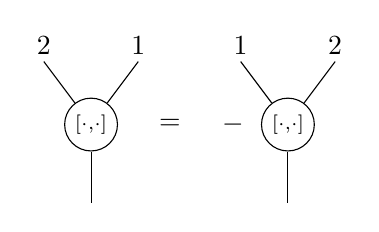
\begin{tikzpicture}[scale=1]

\node[circle,draw,inner sep=2pt] (b) at (0,0) {${\scriptstyle[\cdot,\cdot]}$};
\draw (-0.6,0.8)--(b);
\draw (0.6,0.8)--(b);
\draw (b)--(0,-1);
\node at (-0.6,1) {$2$};
\node at (0.6,1) {$1$};
\node at (1,0) {$=$};
\node at (1.8,0) {$-$};
\begin{scope}[shift={(2.5,0)}]
\node[circle,draw,inner sep=2pt] (b) at (0,0) {${\scriptstyle[\cdot,\cdot]}$};
\draw (-0.6,0.8)--(b);
\draw (0.6,0.8)--(b);
\draw (b)--(0,-1);
\node at (-0.6,1) {$1$};
\node at (0.6,1) {$2$};
\end{scope}

\end{tikzpicture}
\]
The Jacobi relation is thus represented by 
\[
\small
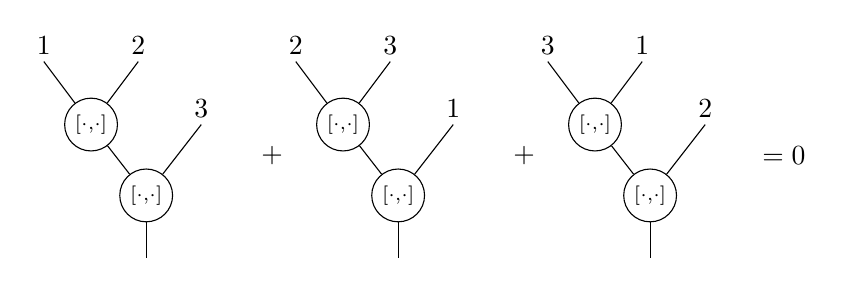
\begin{tikzpicture}[scale=1]

\node[circle,draw,inner sep=2pt] (b1) at (0,0) {$\scriptstyle[\cdot,\cdot]$};
\draw (b1)--(0,-0.8);

\node[circle,draw,inner sep=2pt] (a1) at (-0.7,0.9) {$\scriptstyle[\cdot,\cdot]$};
\draw (a1)--(b1);
\draw (-1.3,1.7)--(a1);
\draw (-0.1,1.7)--(a1);

\draw (0.7,0.9)--(b1);

\node at (-1.3,1.9) {$1$};
\node at (-0.1,1.9) {$2$};
\node at (0.7,1.1) {$3$};

\node at (1.6,0.5) {$+$};

\begin{scope}[shift={(3.2,0)}]

\node[circle,draw,inner sep=2pt] (b2) at (0,0) {$\scriptstyle[\cdot,\cdot]$};
\draw (b2)--(0,-0.8);

\node[circle,draw,inner sep=2pt] (a2) at (-0.7,0.9) {$\scriptstyle[\cdot,\cdot]$};
\draw (a2)--(b2);
\draw (-1.3,1.7)--(a2);
\draw (-0.1,1.7)--(a2);

\draw (0.7,0.9)--(b2);

\node at (-1.3,1.9) {$2$};
\node at (-0.1,1.9) {$3$};
\node at (0.7,1.1) {$1$};

\end{scope}

\node at (4.8,0.5) {$+$};

\begin{scope}[shift={(6.4,0)}]

\node[circle,draw,inner sep=2pt] (b3) at (0,0) {$\scriptstyle[\cdot,\cdot]$};
\draw (b3)--(0,-0.8);

\node[circle,draw,inner sep=2pt] (a3) at (-0.7,0.9) {$\scriptstyle[\cdot,\cdot]$};
\draw (a3)--(b3);
\draw (-1.3,1.7)--(a3);
\draw (-0.1,1.7)--(a3);

\draw (0.7,0.9)--(b3);

\node at (-1.3,1.9) {$3$};
\node at (-0.1,1.9) {$1$};
\node at (0.7,1.1) {$2$};

\end{scope}

\node at (8.1,0.5) {$=0$};

\end{tikzpicture}
\]
whence the post-Lie relations \eqref{eq:postlie:1} and \eqref{eq:postlie:2} are respectively described by
\[
\footnotesize
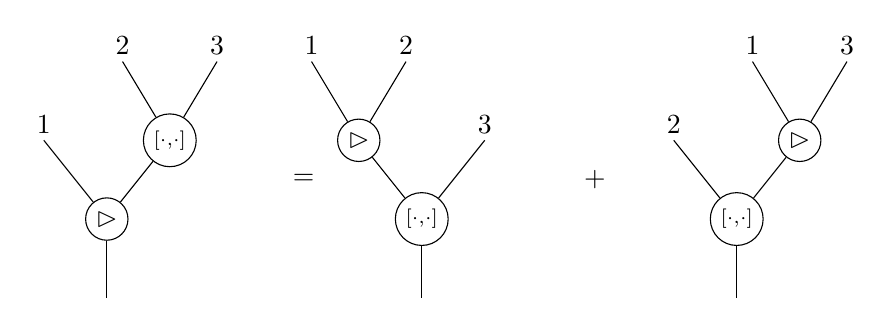
\begin{tikzpicture}[scale=1]

\node[circle,draw,inner sep=2pt] (w) at (0,0) {$\wt$};

\node[circle,draw,inner sep=2pt] (b) at (0.8,1) {$\scriptstyle[\cdot,\cdot]$};

\draw (w) -- (0,-1);
\draw (-0.8,1) -- (w);
\draw (b) -- (w);
\draw (0.2,2) -- (b);
\draw (1.4,2) -- (b);

\node at (-0.8,1.2) {$1$};
\node at (0.2,2.2) {$2$};
\node at (1.4,2.2) {$3$};

\node at (2.5,0.5) {$=$};


\begin{scope}[shift={(4,0)}]

\node[circle,draw,inner sep=2pt] (b1) at (0,0) {$\scriptstyle[\cdot,\cdot]$};

\node[circle,draw,inner sep=2pt] (w1) at (-0.8,1) {$\wt$};

\draw (b1) -- (0,-1);
\draw (w1) -- (b1);
\draw (0.8,1) -- (b1);

\draw (-1.4,2) -- (w1);
\draw (-0.2,2) -- (w1);

\node at (-1.4,2.2) {$1$};
\node at (-0.2,2.2) {$2$};
\node at (0.8,1.2) {$3$};

\end{scope}

\node at (6.2,0.5) {$+$};

\begin{scope}[shift={(8,0)}]

\node[circle,draw,inner sep=2pt] (b2) at (0,0) {$\scriptstyle[\cdot,\cdot]$};

\node[circle,draw,inner sep=2pt] (w2) at (0.8,1) {$\wt$};

\draw (b2) -- (0,-1);
\draw (-0.8,1) -- (b2);
\draw (w2) -- (b2);

\draw (0.2,2) -- (w2);
\draw (1.4,2) -- (w2);

\node at (-0.8,1.2) {$2$};
\node at (0.2,2.2) {$1$};
\node at (1.4,2.2) {$3$};

\end{scope}

\end{tikzpicture}
\]
and 
\[
\small
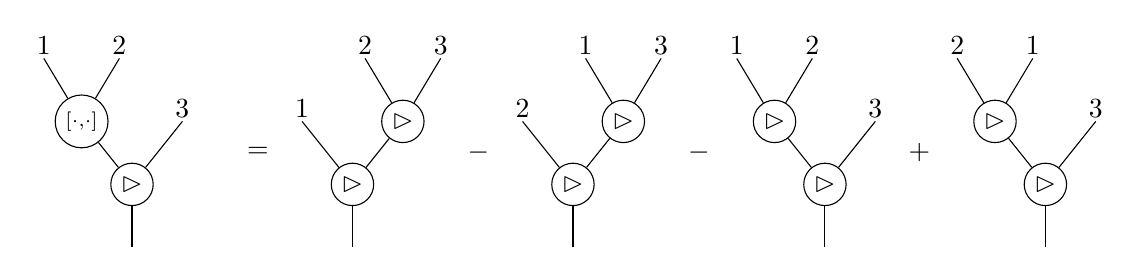
\begin{tikzpicture}[scale=0.8]


\node[circle,draw,inner sep=2pt] (w) at (0,0) {$\wt$};

\node[circle,draw,inner sep=2pt] (b) at (-0.8,1)
{$\scriptstyle[\cdot,\cdot]$};

\draw (w)--(0,-1);

\draw (b)--(w);
\draw (0.8,1)--(w);

\draw (-1.4,2)--(b);
\draw (-0.2,2)--(b);

\node at (-1.4,2.2) {$1$};
\node at (-0.2,2.2) {$2$};
\node at (0.8,1.2) {$3$};

\node at (2,0.5) {$=$};


\begin{scope}[shift={(3.5,0)}]

\node[circle,draw,inner sep=2pt] (w1) at (0,0) {$\wt$};

\node[circle,draw,inner sep=2pt] (w11) at (0.8,1) {$\wt$};

\draw (w1)--(0,-1);

\draw (-0.8,1)--(w1);
\draw (w11)--(w1);

\draw (0.2,2)--(w11);
\draw (1.4,2)--(w11);

\node at (-0.8,1.2) {$1$};
\node at (0.2,2.2) {$2$};
\node at (1.4,2.2) {$3$};

\end{scope}

\node at (5.5,0.5) {$-$};


\begin{scope}[shift={(7,0)}]

\node[circle,draw,inner sep=2pt] (w2) at (0,0) {$\wt$};

\node[circle,draw,inner sep=2pt] (w22) at (0.8,1) {$\wt$};

\draw (w2)--(0,-1);

\draw (-0.8,1)--(w2);
\draw (w22)--(w2);

\draw (0.2,2)--(w22);
\draw (1.4,2)--(w22);

\node at (-0.8,1.2) {$2$};
\node at (0.2,2.2) {$1$};
\node at (1.4,2.2) {$3$};

\end{scope}

\node at (9,0.5) {$-$};


\begin{scope}[shift={(11,0)}]

\node[circle,draw,inner sep=2pt] (w3) at (0,0) {$\wt$};

\node[circle,draw,inner sep=2pt] (w33) at (-0.8,1) {$\wt$};

\draw (w3)--(0,-1);

\draw (w33)--(w3);
\draw (0.8,1)--(w3);

\draw (-1.4,2)--(w33);
\draw (-0.2,2)--(w33);

\node at (-1.4,2.2) {$1$};
\node at (-0.2,2.2) {$2$};
\node at (0.8,1.2) {$3$};

\end{scope}

\node at (12.5,0.5) {$+$};


\begin{scope}[shift={(14.5,0)}]

\node[circle,draw,inner sep=2pt] (w4) at (0,0) {$\wt$};

\node[circle,draw,inner sep=2pt] (w44) at (-0.8,1) {$\wt$};

\draw (w4)--(0,-1);

\draw (w44)--(w4);
\draw (0.8,1)--(w4);

\draw (-1.4,2)--(w44);
\draw (-0.2,2)--(w44);

\node at (-1.4,2.2) {$2$};
\node at (-0.2,2.2) {$1$};
\node at (0.8,1.2) {$3$};

\end{scope}

\end{tikzpicture}
\]
Finally, relations \eqref{eq:infpostlie:1} and \eqref{eq:infpostlie:2} are respectively represented by 
\[
\footnotesize
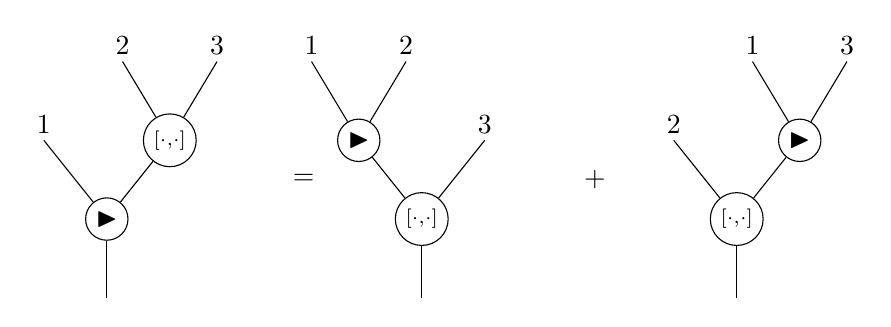
\begin{tikzpicture}[scale=1]


\node[circle,draw,inner sep=2pt] (w) at (0,0) {$\bt$};

\node[circle,draw,inner sep=2pt] (b) at (0.8,1) {$\scriptstyle[\cdot,\cdot]$};

\draw (w) -- (0,-1);
\draw (-0.8,1) -- (w);
\draw (b) -- (w);
\draw (0.2,2) -- (b);
\draw (1.4,2) -- (b);

\node at (-0.8,1.2) {$1$};
\node at (0.2,2.2) {$2$};
\node at (1.4,2.2) {$3$};

\node at (2.5,0.5) {$=$};


\begin{scope}[shift={(4,0)}]

\node[circle,draw,inner sep=2pt] (b1) at (0,0) {$\scriptstyle[\cdot,\cdot]$};

\node[circle,draw,inner sep=2pt] (w1) at (-0.8,1) {$\bt$};

\draw (b1) -- (0,-1);
\draw (w1) -- (b1);
\draw (0.8,1) -- (b1);

\draw (-1.4,2) -- (w1);
\draw (-0.2,2) -- (w1);

\node at (-1.4,2.2) {$1$};
\node at (-0.2,2.2) {$2$};
\node at (0.8,1.2) {$3$};

\end{scope}

\node at (6.2,0.5) {$+$};


\begin{scope}[shift={(8,0)}]

\node[circle,draw,inner sep=2pt] (b2) at (0,0) {$\scriptstyle[\cdot,\cdot]$};

\node[circle,draw,inner sep=2pt] (w2) at (0.8,1) {$\bt$};

\draw (b2) -- (0,-1);
\draw (-0.8,1) -- (b2);
\draw (w2) -- (b2);

\draw (0.2,2) -- (w2);
\draw (1.4,2) -- (w2);

\node at (-0.8,1.2) {$2$};
\node at (0.2,2.2) {$1$};
\node at (1.4,2.2) {$3$};

\end{scope}

\end{tikzpicture}
\]
and
\[
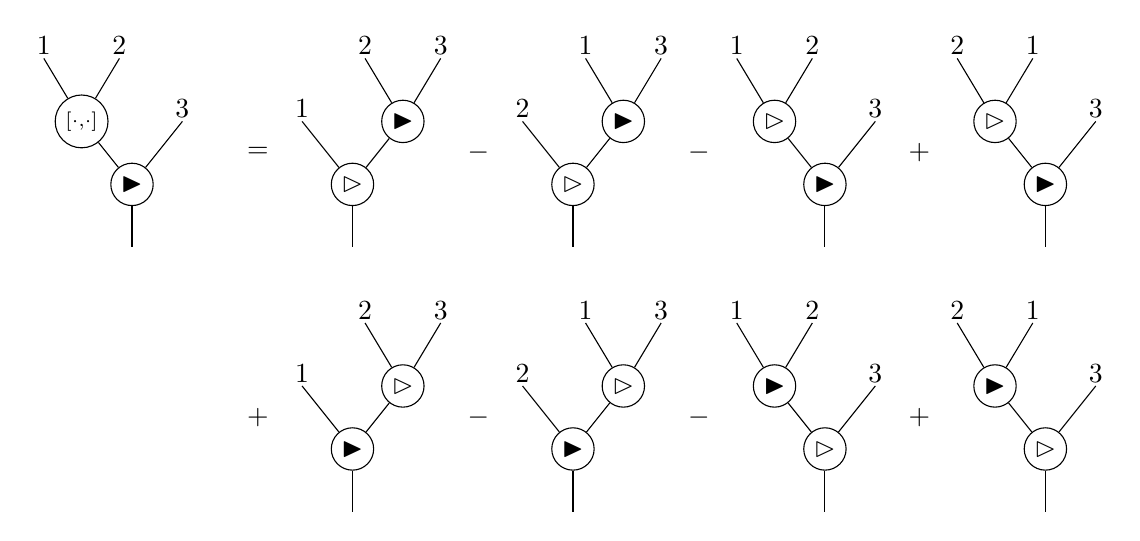
\begin{tikzpicture}[scale=0.8]


\node[circle,draw,inner sep=2pt] (bt0) at (0,0) {$\bt$};
\node[circle,draw,inner sep=2pt] (br) at (-0.8,1)
{$\scriptstyle[\cdot,\cdot]$};

\draw (bt0)--(0,-1);
\draw (br)--(bt0);
\draw (0.8,1)--(bt0);

\draw (-1.4,2)--(br);
\draw (-0.2,2)--(br);

\node at (-1.4,2.2) {$1$};
\node at (-0.2,2.2) {$2$};
\node at (0.8,1.2) {$3$};

\node at (2,0.5) {$=$};


\begin{scope}[shift={(3.5,0)}]

\node[circle,draw,inner sep=2pt] (w1) at (0,0) {$\wt$};
\node[circle,draw,inner sep=2pt] (b1) at (0.8,1) {$\bt$};

\draw (w1)--(0,-1);
\draw (-0.8,1)--(w1);
\draw (b1)--(w1);
\draw (0.2,2)--(b1);
\draw (1.4,2)--(b1);

\node at (-0.8,1.2) {$1$};
\node at (0.2,2.2) {$2$};
\node at (1.4,2.2) {$3$};

\end{scope}

\node at (5.5,0.5) {$-$};


\begin{scope}[shift={(7,0)}]

\node[circle,draw,inner sep=2pt] (w2) at (0,0) {$\wt$};
\node[circle,draw,inner sep=2pt] (b2) at (0.8,1) {$\bt$};

\draw (w2)--(0,-1);
\draw (-0.8,1)--(w2);
\draw (b2)--(w2);
\draw (0.2,2)--(b2);
\draw (1.4,2)--(b2);

\node at (-0.8,1.2) {$2$};
\node at (0.2,2.2) {$1$};
\node at (1.4,2.2) {$3$};

\end{scope}

\node at (9,0.5) {$-$};


\begin{scope}[shift={(11,0)}]

\node[circle,draw,inner sep=2pt] (b3) at (0,0) {$\bt$};
\node[circle,draw,inner sep=2pt] (w3) at (-0.8,1) {$\wt$};

\draw (b3)--(0,-1);
\draw (w3)--(b3);
\draw (0.8,1)--(b3);
\draw (-1.4,2)--(w3);
\draw (-0.2,2)--(w3);

\node at (-1.4,2.2) {$1$};
\node at (-0.2,2.2) {$2$};
\node at (0.8,1.2) {$3$};

\end{scope}

\node at (12.5,0.5) {$+$};


\begin{scope}[shift={(14.5,0)}]

\node[circle,draw,inner sep=2pt] (b4) at (0,0) {$\bt$};
\node[circle,draw,inner sep=2pt] (w4) at (-0.8,1) {$\wt$};

\draw (b4)--(0,-1);
\draw (w4)--(b4);
\draw (0.8,1)--(b4);
\draw (-1.4,2)--(w4);
\draw (-0.2,2)--(w4);

\node at (-1.4,2.2) {$2$};
\node at (-0.2,2.2) {$1$};
\node at (0.8,1.2) {$3$};

\end{scope}


\begin{scope}[shift={(0,-4.2)}] 
\node at (2,0.5) {$+$};

\begin{scope}[shift={(3.5,0)}]

\node[circle,draw,inner sep=2pt] (b1) at (0,0) {$\bt$};
\node[circle,draw,inner sep=2pt] (w1) at (0.8,1) {$\wt$};

\draw (b1)--(0,-1);
\draw (-0.8,1)--(b1);
\draw (w1)--(b1);
\draw (0.2,2)--(w1);
\draw (1.4,2)--(w1);

\node at (-0.8,1.2) {$1$};
\node at (0.2,2.2) {$2$};
\node at (1.4,2.2) {$3$};

\end{scope}

\node at (5.5,0.5) {$-$};

\begin{scope}[shift={(7,0)}]

\node[circle,draw,inner sep=2pt] (b2) at (0,0) {$\bt$};
\node[circle,draw,inner sep=2pt] (w2) at (0.8,1) {$\wt$};

\draw (b2)--(0,-1);
\draw (-0.8,1)--(b2);
\draw (w2)--(b2);
\draw (0.2,2)--(w2);
\draw (1.4,2)--(w2);

\node at (-0.8,1.2) {$2$};
\node at (0.2,2.2) {$1$};
\node at (1.4,2.2) {$3$};

\end{scope}

\node at (9,0.5) {$-$};

\begin{scope}[shift={(11,0)}]

\node[circle,draw,inner sep=2pt] (w3) at (0,0) {$\wt$};
\node[circle,draw,inner sep=2pt] (b3) at (-0.8,1) {$\bt$};

\draw (w3)--(0,-1);
\draw (b3)--(w3);
\draw (0.8,1)--(w3);
\draw (-1.4,2)--(b3);
\draw (-0.2,2)--(b3);

\node at (-1.4,2.2) {$1$};
\node at (-0.2,2.2) {$2$};
\node at (0.8,1.2) {$3$};

\end{scope}

\node at (12.5,0.5) {$+$};

\begin{scope}[shift={(14.5,0)}]

\node[circle,draw,inner sep=2pt] (w4) at (0,0) {$\wt$};
\node[circle,draw,inner sep=2pt] (b4) at (-0.8,1) {$\bt$};

\draw (w4)--(0,-1);
\draw (b4)--(w4);
\draw (0.8,1)--(w4);
\draw (-1.4,2)--(b4);
\draw (-0.2,2)--(b4);

\node at (-1.4,2.2) {$2$};
\node at (-0.2,2.2) {$1$};
\node at (0.8,1.2) {$3$};

\end{scope}

\end{scope}

\end{tikzpicture}
\]

\begin{theorem}\label{thm:IPL}
The operad $\mathcal{IPL}$ is Koszul.
\end{theorem}
\begin{proof}
We shall use Theorem \ref{theorem-Koszulity} and follow the same line of thought used in \cite[6.1]{DG} for the proof of the Koszulity of $\mathcal{PL}$. Consider the operad $\mathcal{L}$ of Lie algebras, and the operad $\mathcal{M}_2 := \mathcal{F}(\wt,\bt)$. It is clear that the latter is Koszul, while it is well-known that $\mathcal{L}$ is Koszul, see e.g.\ \cite[13.2.6]{LodayVallette}. Set $\mathcal{V}=\Bbbk\langle [\cdot,\cdot]\rangle$, $\mathcal{W}=\Bbbk\langle \wt,\bt \rangle$, and let $\mathcal{R}=\{ \mathrm{J}\}$, where $\mathrm{J}$ denotes the Jacobi identity. Consider the $\mathbb{S}$-modules maps $s,d$ of the form \eqref{eq:filtered-law-one}-\eqref{eq:filtered-law-two} given by $s=0$ and 
\begin{align*}
d(\wt \circ_2 [\cdot,\cdot] ) &=  [\cdot,\cdot]\circ_1 \wt + ([\cdot,\cdot]\circ_2\wt ) \cdot(12)\\
d(\wt \circ_1 [\cdot,\cdot]  ) &= (\wt \circ_2 \wt) \cdot (\mathrm{id}_{\mathbb{S}_3} - (12)) + (\wt \circ_1 \wt) \cdot ((12) -\mathrm{id}_{\mathbb{S}_3} ) \\
d(\bt \circ_2 [\cdot,\cdot] ) &=  [\cdot,\cdot]\circ_1 \bt + ([\cdot,\cdot]\circ_2\bt ) \cdot(12)\\
d(\bt\circ_1[\cdot,\cdot]  ) &= (\wt \circ_2 \bt + \bt \circ_2 \wt) \cdot (\mathrm{id}_{\mathbb{S}_3} - (12)) + (\wt \circ_1 \bt + \bt \circ_1 \wt) \cdot ((12) -\mathrm{id}_{\mathbb{S}_3} )
\end{align*}
which we can write in a more algebraic fashion as
\begin{align*}
d(x \wt [y,z]) &= [x \wt y,z] + [y,x \wt z] \\
d([x,y] \wt z )&= x \wt (y \wt z) - y \wt (x \wt z) - (x \wt y) \wt z + (y \wt x) \wt z \\
d(x \bt [y,z]) &= [x \bt y,z] + [y,x \bt z] \\
d([x,y] \bt z) &= \R(x,y,z) - \R(y,x,z) - \L(x,y,z) + \L(y,x,z).
\end{align*}
Employing the same notations of Definition \ref{definition-filtered-law}, we thus have $\mathcal{D} = \{ \mathrm{PL}_1, \mathrm{PL}_2, \mathrm{IPL}_1, \mathrm{IPL}_2\}$,  $\mathcal{G}= \mathcal{R} = \{ \mathrm{J}\}$, and $\mathcal{S}= \emptyset$, where $\mathrm{PL}_1, \mathrm{PL}_2, \mathrm{IPL}_1, \mathrm{IPL}_2$ denotes respectively the relations \eqref{eq:postlie:1}, \eqref{eq:postlie:2}, \eqref{eq:infpostlie:1}, \eqref{eq:infpostlie:2}. Therefore, we have that $\mathcal{E} \cong \mathcal{IPL}$. If the corresponding map $\xi_3$ is an isomorphism, then the pair $(s,d)$ defines a filtered distributive law; consequently, we can apply Theorem \ref{theorem-Koszulity} to conclude that $\mathcal{IPL}$ is Koszul, and, in particular, $\mathcal{IPL} \cong \mathcal{L} \circ \mathcal{M}_2$ as $\mathbb{S}$-modules.
To verify that the surjective map $\xi_{3}$ is injective, it remains to check that the following critical pairs\footnote{The term \emph{critical pair} is borrowed from the theory of Gr\"obner basis for quadratic operads. Since the computations that follow are identical to those required to show Koszulity using the Hoffbeck-Dotsenko-Khoroshkin approach, we adopt the same terminology.} are confluent:
\[
[x,y]\bt[z,w],\qquad [[x,y],z]\bt w,\qquad x\bt[[y,z],w]
\]
where we again used an algebraic representation of the corresponding operadic elements.
We observe that the third one follows as in the case of post-Lie algebras, thus, we only have to check the first two. 
We first check the critical pair $[x,y]\bt[z,w]$. The first path (using first the rule \eqref{eq:infpostlie:2}) gives
\begingroup
\allowdisplaybreaks
\begin{align*}
[x,y] \bt [z,w] &= \R(x,y,[z,w]) - \R(y,x,[z,w]) - \L(x,y,[x,z]) + \L(y,x,[z,w]) \\
&= x \wt (y \bt [z,w]) + x \bt(y \wt [z,w]) - y \wt (x \bt [z,w]) - y \bt(x \wt [z,w]) \\
& - (x \wt y) \bt[z,w] - (x \bt y) \wt[z,w] + (y \wt x) \bt[z,w] + (y \bt x) \wt[z,w] \\
&= x \wt [y \bt z,w] + x \wt [z, y \bt w] + x \bt [y \wt z,w] + x \bt [z, y \wt w] \\
& - y \wt [x \bt z,w] - y \wt [z, x \bt w] - y \bt [x \wt z,w] - y \bt [z, x \wt w]\\
&- [(x \wt y)\bt z,w] -[z,(x \wt y)\bt w] - [(x \bt y)\wt z,w] -[z,(x \bt y)\wt w] \\
&+  [(y \wt x)\bt z,w] +[z,(y \wt x)\bt w] + [(y \bt x)\wt z,w] +[z,(y \bt x)\wt w]\\
&=[x \wt (y \bt z),w] + [y \bt z, x \wt w] + [x \wt z, y \bt w] + [z, x \wt (y \bt w)]\\
& + [x \bt (y \wt z),w] + [y \wt z, x \bt w] + [x \bt z, y \wt w] + [z, x \bt (y \wt w)]\\
& - [y \wt (x \bt z),w] - [x \bt z,y \wt w ] - [y \wt z , x \bt w] - [z, y \wt (x \bt w)]\\
&- [y \bt (x \wt z),w] - [x \wt z,y \bt w ] - [y \bt z , x \wt w] - [z, y \bt (x \wt w)]\\
&- [(x \wt y)\bt z,w] -[z,(x \wt y)\bt w] - [(x \bt y)\wt z,w] -[z,(x \bt y)\wt w] \\
&+  [(y \wt x)\bt z,w] +[z,(y \wt x)\bt w] + [(y \bt x)\wt z,w] +[z,(y \bt x)\wt w] \\
&= x \wt [y \bt z,w] + x \wt [z, y \bt w] + x \bt [y \wt z,w] + x \bt [z, y \wt w] \\
& - y \wt [x \bt z,w] - y \wt [z, x \bt w] - y \bt [x \wt z,w] - y \bt [z, x \wt w]\\
&- [(x \wt y)\bt z,w] -[z,(x \wt y)\bt w] - [(x \bt y)\wt z,w] -[z,(x \bt y)\wt w] \\
&+  [(y \wt x)\bt z,w] +[z,(y \wt x)\bt w] + [(y \bt x)\wt z,w] +[z,(y \bt x)\wt w]\\
&=[x \wt (y \bt z),w] + [z, x \wt (y \bt w)] + [x \bt (y \wt z),w]  + [z, x \bt (y \wt w)]\\
& - [y \wt (x \bt z),w] - [z, y \wt (x \bt w)]- [y \bt (x \wt z),w]  - [z, y \bt (x \wt w)]\\
&- [(x \wt y)\bt z,w] -[z,(x \wt y)\bt w] - [(x \bt y)\wt z,w] -[z,(x \bt y)\wt w] \\
&+  [(y \wt x)\bt z,w] +[z,(y \wt x)\bt w] + [(y \bt x)\wt z,w] +[z,(y \bt x)\wt w] .
\end{align*}
\endgroup
The second path (using first the rule \eqref{eq:infpostlie:1}) gives
\begingroup
\allowdisplaybreaks
\begin{align*}
[x,y] \bt [z,w] &= [[x,y] \bt z, w] + [z, [x,y] \bt w] \\
&= [\R(x,y,z),w] - [\R(y,x,z),w] - [\L(x,y,z),w] + [\L(y,x,z),w] \\
& + [z,\R(x,y,w)] - [z,\R(y,x,w)] - [z, \L(x,y,w)] + [z,\L(y,x,w)]\\
&= [x \wt (y \bt z),w] + [x \bt (y \wt z),w] - [y \wt (x \bt z),w] - [y \bt (x \wt z),w]\\
&- [(x \wt y) \bt z,w] - [(x \bt y)\wt z,w] + [(y \wt x) \bt z,w] + [(y \bt x)\wt z,w]\\
& + [z, x \wt (y \bt w)] +  [z, x \bt (y \wt w)] - [z, y \wt (x \bt w)] - [z, y \bt (x \wt w)]\\
& - [z, (x \wt y) \bt w] - [z, (x \bt y) \wt w] + [z, (y \wt x) \bt w] + [z, (y \bt x) \wt w].
\end{align*}
A careful but easy check shows that both paths give the same expansion.
\endgroup

\medskip\medskip
Next, we check the critical pair $[[x,y],z]\bt w$, which turns out to be the most intricate case. We will use \eqref{eq:postlie:1},\eqref{eq:postlie:2},\eqref{eq:infpostlie:1} and \eqref{eq:infpostlie:2}, rewritten by using the operators $D_{x}:=x\wt(-)$ and $E_{x}:=x\bt(-)$, and by employing notations $\ab{x}{y} := x\wt y-y\wt x$ and $\abd{x}{y} := x\bt y-y\bt x$. These have the following form:
\begin{align}
D_x[y,z] &= [D_xy,z]+[y,D_xz],\label{PL1'}\\
D_{[x,y]} &= [D_x,D_y]-D_{\ab{x}{y}},\label{PL2'}\\
E_x[y,z] &= [E_xy,z]+[y,E_xz],\label{IPL1'}\\
E_{[x,y]} &= [D_x,E_y]+[E_x,D_y]-E_{\ab{x}{y}}-D_{\abd{x}{y}}\label{IPL2'}.
\end{align} 

We have $[[x,y],z]\bt w = E_{[[x,y],z]}(w)$, hence we study $E_{[[x,y],z]}$. \medskip

The first path $(A)$ uses \eqref{IPL2'}. Hence, we have
\begin{equation}\label{eq1}
E_{[[x,y],z]}\overset{\eqref{IPL2'}}{=}\underbrace{[D_{[x,y]},E_z]+[E_{[x,y]},D_z]}+(\underbrace{
   -E_{\ab{[x,y]}{z}}-D_{\abd{[x,y]}{z}}})=:\mathcal{P}_A+\mathcal{S}_A .
\end{equation}
We compute
\begin{align*}
[D_{[x,y]},E_z] &\overset{\eqref{PL2'}}{=} \bigl[[D_x,D_y],E_z\bigr]-[D_{\ab{x}{y}},E_z],\\
[E_{[x,y]},D_z] &\overset{\eqref{IPL2'}}{=} \bigl[[D_x,E_y],D_z\bigr]+\bigl[[E_x,D_y],D_z\bigr]-[E_{\ab{x}{y}},D_z]-[D_{\abd{x}{y}},D_z].
\end{align*}
We also have
\begin{align*}
\ab{[x,y]}{z}  &= [x,y]\wt z-z\wt[x,y]\overset{\eqref{PL1'}}{=} D_{[x,y]}z-\bigl([z\wt x,y]+[x,z\wt y]\bigr),\\
\abd{[x,y]}{z} &= [x,y]\bt z-z\bt[x,y]\overset{\eqref{IPL1'}}{=} E_{[x,y]}z-\bigl([z\bt x,y]+[x,z\bt y]\bigr),
\end{align*}
so that 
\begin{align*}
  -E_{\ab{[x,y]}{z}}  &= -E_{D_{[x,y]}z}+E_{[z\wt x,\,y]}+E_{[x,\,z\wt y]},\\
  -D_{\abd{[x,y]}{z}} &= -D_{E_{[x,y]}z}+D_{[z\bt x,\,y]}+D_{[x,\,z\bt y]}.
\end{align*}
Furthermore, we have
\begin{align*}
E_{[z\wt x,y]} &\overset{\eqref{IPL2'}}{=} [D_{z\wt x},E_y]+[E_{z\wt x},D_y]-E_{\ab{z\wt x}{y}}-D_{\abd{z\wt x}{y}},\\
E_{[x,z\wt y]} &\overset{\eqref{IPL2'}}{=}[D_x,E_{z\wt y}]+[E_x,D_{z\wt y}]-E_{\ab{x}{z\wt y}}-D_{\abd{x}{z\wt y}},\\
D_{[z\bt x,y]} &\overset{\eqref{PL2'}}{=} [D_{z\bt x},D_y]-D_{\ab{z\bt x}{y}},\\
D_{[x,z\bt y]} &\overset{\eqref{PL2'}}{=} [D_x,D_{z\bt y}]-D_{\ab{x}{z\bt y}}.
\end{align*}
We also compute
\begin{align*}
D_{[x,y]}z &\overset{\eqref{PL2'}}{=} x\wt(y\wt z)-y\wt(x\wt z)-\ab{x}{y}\wt z,\\
E_{[x,y]}z &\overset{\eqref{IPL2'}}{=} x\wt(y\bt z)+x\bt(y\wt z)-y\wt(x\bt z)-y\bt(x\wt z)-\abd{x}{y}\wt z-\ab{x}{y}\bt z,
\end{align*}
hence \eqref{eq1} reads $E_{[[x,y],z]}=\mathcal{P}_A+\mathcal{S}_A$, where:
\begin{align*}
\mathcal P_A&= \underbrace{\bigl[[D_x,D_y],E_z\bigr]+\bigl[[D_x,E_y],D_z\bigr]+\bigl[[E_x,D_y],D_z\bigr]}_{\text{(i)}}\quad\underbrace{-\,[D_{\ab{x}{y}},E_z]-[E_{\ab{x}{y}},D_z]-[D_{\abd{x}{y}},D_z]}_{\text{(ii)}}\\[2pt]
&\quad \underbrace{+\,[D_{z\wt x},E_y]+[E_{z\wt x},D_y]+[D_{z\bt x},D_y]+[D_x,E_{z\wt y}]+[E_x,D_{z\wt y}]+[D_x,D_{z\bt y}]}_{\text{(iii)}}\, 
\end{align*}
and 
\begin{align*}
\mathcal S_A &= -E_{\,D_{[x,y]}z\,+\,\ab{z\wt x}{y}\,+\,\ab{x}{z\wt y}}-D_{\,E_{[x,y]}z\,+\,\abd{z\wt x}{y}+\abd{x}{z\wt y}+\ab{z\bt x}{y}+\ab{x}{z\bt y}} .
\end{align*}

\medskip
The second path $(B)$ uses Jacobi. Hence, we have $ E_{[[x,y],z]}=E_{[x,[y,z]]}-E_{[y,[x,z]]}$. We compute the first addend, the second will be obtained by interchanging $x$ with $y$. We have
\begin{equation}\label{eq2}
E_{[x,[y,z]]}\overset{\eqref{IPL2'}}{=}[D_x,E_{[y,z]}]+[E_x,D_{[y,z]}]+(-E_{\ab{x}{[y,z]}}-D_{\abd{x}{[y,z]}}).
\end{equation}
We will denote by $\mathcal{P}_{B}$ the first two addends of \eqref{eq2} together with the other two coming from interchanging $x$ with $y$, and by $\mathcal{S}_{B}$ the third and fourth addends and the two coming from interchanging $x$ with $y$.


\begin{align*}
[D_x,E_{[y,z]}] &\overset{\eqref{IPL2'}}{=}\bigl[D_x,[D_y,E_z]\bigr]+\bigl[D_x,[E_y,D_z]\bigr]-[D_x,E_{\ab{y}{z}}]-[D_x,D_{\abd{y}{z}}],\\
  [E_x,D_{[y,z]}] &\overset{\eqref{PL2'}}{=} \bigl[E_x,[D_y,D_z]\bigr]-[E_x,D_{\ab{y}{z}}].
\end{align*}
We also compute 
\begin{align*}
  \ab{x}{[y,z]}  &\overset{\eqref{PL1'}}{=} x\wt[y,z]-[y,z]\wt x=[x\wt y,z]+[y,x\wt z]-D_{[y,z]}x,\\
  \abd{x}{[y,z]} &\overset{\eqref{IPL1'}}{=} x\bt[y,z]-[y,z]\bt x=[x\bt y,z]+[y,x\bt z]-E_{[y,z]}x,
\end{align*}
so that
\begin{align*}
  -E_{\ab{x}{[y,z]}}  &= -E_{[x\wt y,z]}-E_{[y,x\wt z]}+E_{D_{[y,z]}x},\\
  -D_{\abd{x}{[y,z]}} &= -D_{[x\bt y,z]}-D_{[y,x\bt z]}+D_{E_{[y,z]}x}.
\end{align*}
Moreover, we have
\begin{align*}
E_{[x\wt y,z]} &\overset{\eqref{IPL2'}}{=} [D_{x\wt y},E_z]+[E_{x\wt y},D_z]-E_{\ab{x\wt y}{z}}-D_{\abd{x\wt y}{z}},\\
E_{[y,x\wt z]} &\overset{\eqref{IPL2'}}{=}[D_y,E_{x\wt z}]+[E_y,D_{x\wt z}]-E_{\ab{y}{x\wt z}}-D_{\abd{y}{x\wt z}},\\
D_{[x\bt y,z]} &\overset{\eqref{PL2'}}{=} [D_{x\bt y},D_z]-D_{\ab{x\bt y}{z}},\\
D_{[y,x\bt z]} &\overset{\eqref{PL2'}}{=} [D_y,D_{x\bt z}]-D_{\ab{y}{x\bt z}} .
\end{align*}
Therefore, we get
\begin{align*}
\mathcal P_B&= \Bigl\{\bigl[D_x,[D_y,E_z]\bigr]+\bigl[D_x,[E_y,D_z]\bigr]+\bigl[E_x,[D_y,D_z]\bigr]\\
&\qquad -[D_x,E_{\ab{y}{z}}]-[D_x,D_{\abd{y}{z}}]-[E_x,D_{\ab{y}{z}}]\\
&\qquad -[D_{x\wt y},E_z]-[E_{x\wt y},D_z]-[D_{x\bt y},D_z]\\
  &\qquad -[D_y,E_{x\wt z}]-[E_y,D_{x\wt z}]-[D_y,D_{x\bt z}]
     \Bigr\}-\bigl(x\leftrightarrow y\bigr),
\end{align*}
and
\[
  \mathcal S_B
  = E_{\,\Pi(x,y)-\Pi(y,x)}\;+\;D_{\,\Pi^{\bullet}(x,y)-\Pi^{\bullet}(y,x)},
\]
where
\begin{align*}
\Pi(x,y)&:= D_{[y,z]}x+\ab{x\wt y}{z}+\ab{y}{x\wt z},\\
\Pi^{\bullet}(x,y)&:= E_{[y,z]}x+\abd{x\wt y}{z}+\abd{y}{x\wt z}+\ab{x\bt y}{z}+\ab{y}{x\bt z}.
\end{align*}
We now compare path $(A)$ with path $(B)$. By Jacobi in $\mathrm{End}$, we have that the addends in $(i)$ of $\mathcal{P}_{A}$ are :
\begin{align*}
\bigl[[D_x,D_y],E_z\bigr] &= \bigl[D_x,[D_y,E_z]\bigr]-\bigl[D_y,[D_x,E_z]\bigr],\\
\bigl[[D_x,E_y],D_z\bigr] &= \bigl[D_x,[E_y,D_z]\bigr]-\bigl[E_y,[D_x,D_z]\bigr],\\
\bigl[[E_x,D_y],D_z\bigr] &= \bigl[E_x,[D_y,D_z]\bigr]-\bigl[D_y,[E_x,D_z]\bigr].
\end{align*}
The six terms on the right are exactly the first three in $\mathcal{P}_{B}$ and the three obtained by interchanging $x$ with $y$. From the third line of $\mathcal{P}_{B}$ with the corresponding terms obtained by interchanging $x$ with $y$, we get
\[
-[D_{x\wt y-y\wt x},E_z]-[E_{x\wt y-y\wt x},D_z]-[D_{x\bt y-y\bt x},D_z]=-[D_{\ab{x}{y}},E_z]-[E_{\ab{x}{y}},D_z]-[D_{\abd{x}{y}},D_z],
\]
which is $(ii)$ in $\mathcal{P}_{A}$. From the second line of $\mathcal{P}_{B}$ with the corresponding terms obtained interchanging $x$ with $y$ we get
\begin{align*}
&-[D_x,E_{y\wt z}]+[D_x,E_{z\wt y}]-[D_x,D_{y\bt z}]+[D_x,D_{z\bt y}]-[E_x,D_{y\wt z}]+[E_x,D_{z\wt y}]\\&+[D_y,E_{x\wt z}]-[D_y,E_{z\wt x}]+[D_y,D_{x\bt z}]-[D_y,D_{z\bt x}]+[E_y,D_{x\wt z}]-[E_y,D_{z\wt x}],
\end{align*}
while the fourth line of $\mathcal{P}_{B}$ with the corresponding terms obtained interchanging $x$ with $y$ gives
\[
-[D_y,E_{x\wt z}]-[E_y,D_{x\wt z}]-[D_y,D_{x\bt z}]\;+\;[D_x,E_{y\wt z}]+[E_x,D_{y\wt z}]+[D_x,D_{y\bt z}] .
\]
Summing with the previous one, it remains
\[
[D_x,E_{z\wt y}]+[D_x,D_{z\bt y}]+[E_x,D_{z\wt y}]-[D_y,E_{z\wt x}]-[D_y,D_{z\bt x}]-[E_y,D_{z\wt x}]
\]
which is $(iii)$ in $\mathcal{P}_{A}$. We have shown that $\mathcal{P}_{A}=\mathcal{P}_{B}$.

From the relations for post-Lie algebras \cite[Theorem 6.1]{DG}, we already know that 
\[
-D_{[x,y]}z-\ab{z\wt x}{y}-\ab{x}{z\wt y}=\Pi(x,y)-\Pi(y,x).
\]
Finally, we have

\begin{align*}
-E_{[x,y]}z-&\abd{z\wt x}{y}-\abd{x}{z\wt y}-\ab{z\bt x}{y}-\ab{x}{z\bt y}\\
&\overset{\eqref{IPL2'}}{=}-x\wt(y\bt z)-x\bt(y\wt z)+y\wt(x\bt z)+y\bt(x\wt z)\\
&+(x\bt y)\wt z-(y\bt x)\wt z+(x\wt y)\bt z-(y\wt x)\bt z\\
&-(z\wt x)\bt y+y\bt(z\wt x)-x\bt(z\wt y)+(z\wt y)\bt x\\
&-(z\bt x)\wt y+y\wt(z\bt x)-x\wt(z\bt y)+(z\bt y)\wt x\\&=\Pi^{\bullet}(x,y)-\Pi^{\bullet}(y,x).
\end{align*}
Therefore, $\mathcal{S}_{A}=\mathcal{S}_{B}$. Hence, all critical pairs are confluent, and $\xi_3$ is an isomorphism, concluding the proof. 
\end{proof}

\section{Outlook}\label{sec:outlook}
We conclude this article with a selection of prospective applications of our results that we intend to investigate in the near future. \\ \\
\textbf{Quantization of post-Lie bialgebras}: recall that a Lie bialgebra is a triple $(\mathfrak{b},[\cdot,\cdot],\delta)$, where $(\mathfrak{b},[\cdot,\cdot])$ is a Lie algebra, $(\mathfrak{b},\delta)$ is a Lie coalgebra, and the cocycle condition $\delta([x,y])= x \cdot\delta(y) - y \cdot \delta(x)$ holds for all $x,y \in \mathfrak{b}$. A topological Hopf algebra $(H,\Delta)$ is said to be a quantization of a Lie bialgebra $(\mathfrak{b},[\cdot,\cdot],\delta)$ if there is a Hopf algebra isomorphism $H/\hbar \cdot H \cong \mathrm{U}(\mathfrak{b})$ such that 
\[ \delta(x) = \frac{\Delta(\tilde{x}) - \Delta^{\mathrm{op}}(\tilde{x})}{\hbar} \ \mod \hbar\]
where $\tilde{x}$ is any lift of $x$ in $H$. The problem of quantization of Lie bialgebras was posed by V. Drinfeld \cite{Drinfeld90} and solved by P. Etingof and D. Kazhdan \cite{EK} (see also P. \v{S}evera's solution \cite{Sev}). Since the universal enveloping algebra of a post-Lie algebra carries a natural structure of a post-Hopf algebra (see Theorem \ref{thm:postHopfonuniversalenveloping}), it is natural to ask whether post structures are compatible with quantization. We expect that, if  $(\mathfrak{b},[\cdot,\cdot],\delta)$ is a Lie bialgebra together with a \emph{compatible} post-Lie structure  $(\mathfrak{b},[\cdot,\cdot],\wt)$, there is a topological post-Hopf algebra $(H,\Delta,\wp)$ quantizing  $(\mathfrak{b},[\cdot,\cdot],\delta)$ and such that the \emph{semiclassical limit} of $\wp$ is $\wt$. \\ \\
\textbf{Infinitesimal post-Lie-Rinehart algebras and post-Hopf algebroids}: two well-established generalisations of the concepts of Lie algebra and Hopf algebra are the well-known notions of Lie-Rinehart algebra \cite{Rinehart} and of Hopf algebroid \cite{Lu}. %(see also \cite{Bohm,Sch} for other different definitions). 
Recently, A. B. Laurent, Y. Li, and Y. Sheng \cite{LLS} proposed an \emph{oid} version of post-Lie algebras and post-Hopf algebras. They also showed that the universal enveloping algebra of a post-Lie-Rinehart algebra carries a natural structure of post-Hopf algebroid, and, moreover, they provided the construction of the free post-Lie-Rinehart algebra. \\
A very natural follow-up would be to use the same techniques to define the notions of infinitesimal post-Lie-Rinehart algebra and infinitesimal post-Hopf algebroid, and to discuss their geometric interpretation.\\ \\
\textbf{Classification of infinitesimal post-Lie algebra structures on $\mathfrak{t}(2,\mathbb{C})$ and $\mathfrak{gl}(2,\mathbb{C})$}: In Section \ref{subsection-inf-post-lie-sl2}, we have classified infinitesimal post-Lie structures on the Lie algebra $\mathfrak{sl}(2)$. Our classification builds upon the earlier classification of post-Lie structures obtained by D. Burde, K. Dekimpe, and K. Vercammen \cite{BDV}. Similar classification results are available for other Lie algebras. For instance, post-Lie structures on the Lie algebra $\mathfrak{t}(2,\mathbb{C})$ of complex upper triangular matrices were classified by X. Tang and Y. Zhang \cite{TZ}, while those on $\mathfrak{gl}(2,\mathbb{C})$ were classified by Y. Sheng and X. Tang \cite{ST}. A natural direction for future research is to use these classifications to determine the corresponding infinitesimal post-Lie structures on $\mathfrak{t}(2,\mathbb{C})$ and $\mathfrak{gl}(2,\mathbb{C})$.\\ \\ 

\noindent\textit{Acknowledgments.} 
A.\ Rivezzi and A.\ Sciandra are members of the ``National Group for Algebraic and Geometric Structures and their Applications'' (GNSAGA-INdAM). A.\ Rivezzi is supported by GA\v{C}R/NCN grant Quantum Geometric Representation Theory and Noncommutative Fibrations 24-11728K.
A. Sciandra is supported by a postdoctoral fellowship at the ULB within the framework of the PDR project ``Reconstruction of modules and algebraic objects from closed and monoidal structures on their representation categories'' funded by the FNRS under the grant number T.0318.25F (PI J. Vercruysse).
T. Weber is supported by the GA\v{C}R
PIF 24-11324I. This publication is based upon work from COST Action CaLISTA CA21109 supported by COST
(European Cooperation in Science and Technology), www.cost.eu.


\addcontentsline{toc}{section}{References}
\begin{thebibliography}{99}

\bibitem{AGV}
I. Angiono, C. Galindo, L. Vendramin, 
\emph{Hopf braces and Yang--Baxter operators}. Proc. Amer. Math. Soc. 145 (2017), no. 5, 1981-1995.

\bibitem{ABSW}
A. Ardizzoni, L. Bottegoni, A. Sciandra, T. Weber, \emph{Infinitesimal braidings and pre-Cartier bialgebras}. 
Commun. Contemp. Math. 27 (5) (2025) 2450029.


\bibitem{BGST}
C. Bai, L. Guo, Y. Sheng, R. Tang, 
\emph{Post-groups, (Lie-)Butcher groups and the Yang--Baxter equation}. Math. Ann. 388 (2024), 3127-3167.

\bibitem{BFFLS}
F. Bayen, M. Flato, C. Fronsdal, A. Lichnerowicz, D. Sternheimer, \emph{Deformation theory and quantization. I. Deformations of symplectic structures}.
Ann. Phys. 111(1), (1978) 61-110.


\bibitem{BournGran}
D. Bourn, M. Gran, 
\emph{Torsion theories in homological categories}. 
J. Algebra 305 (2006), 18-47.

\bibitem{BST}
Y. Bruned, Y. Sheng, R. Tang, \emph{Post-Lie deformations of pre-Lie algebras and their applications in Regularity Structures}. Preprint \hyperlink{https://arxiv.org/abs/2505.00456}{arxiv.org/abs/2505.00456}.

\bibitem{Buch}
B. Buchberger, \emph{An algorithm for finding a basis for the residue class ring of a zero-dimensional polynomial ideal}. Ph.D. thesis, University of Innsbruck, 1965 (German), J. Symb. Comput. 41 (2006), 471-511.

\bibitem{BDV}
D. Burde, K.  Dekimpe, K. Vercammen, 
\emph{Affine actions on Lie groups and post-Lie algebra structures}.  Linear Algebra Appl. 437(5), 1250-1263 (2012).

\bibitem{Catoire}
P. Catoire,
\emph{The Cartier-Quillen-Milnor-Moore theorem in the Post-Hopf case}. Preprint \hyperlink{https://arxiv.org/abs/2401.09116}{arxiv:2401.09116v3}.

\bibitem{CL}
F. Chapoton, M. Livernet, \emph{Pre-Lie algebras and the rooted trees operad}. Int. Math. Res. Not. 8 (2001) 395-408.

\bibitem{CE-FM-K}
C. Curry, K. Ebrahimi-Fard, H. Munthe-Kaas,
\emph{What is a post-Lie algebra and why is it useful in geometric integration}.
Lect. Notes Comput. Sci. Eng. 126 (2019).

\bibitem{DG}
V. Dotsenko, J. Griffin, \emph{Cacti and filtered distributive laws}. Algebr. Geom. Topol. 14, 6 (2015) 3185-3225.

\bibitem{DK}
V. Dotsenko, A. Khoroshkin, \emph{Gr\"obner basis for operads}. Duke Math. J. 153(2) 363-396 (2010). %DOI: 10.1215/00127094-2010-026

\bibitem{DVJ}
V. Dotsenko, M. Vejdemo-Johansson, \emph{Operadic Gr\"obner Bases: An Implementation}. In International Congress on Mathematical Software (pp. 249-252). Berlin, Heidelberg: Springer Berlin Heidelberg.


\bibitem{Drinfeld90}
V. Drinfeld, \emph{On some unsolved problems in quantum group theory}. In Quantum Groups: Proceedings of Workshops held in the Euler International Mathematical Institute, Leningrad, Fall
1990 (pp. 1-8). Berlin, Heidelberg: Springer Berlin Heidelberg.

\bibitem{ELM}
K. Ebrahimi-Fard, A. Lundervold, and H. Z. Munthe-Kaas, 
\emph{On the Lie enveloping algebra of a post-Lie algebra}. J. Lie Theory 25 (2015), no. 4, 1139-1165.

\bibitem{ERSW}
C. Esposito, A. Rivezzi, J. Schnitzer, T. Weber, \emph{Quantization of infinitesimal braidings and pre-Cartier quasi-bialgebras}. J. Lond. Math. Soc. 113, 3 (2026).

\bibitem{EK}
P. Etingof, D. Kazhdan, \emph{Quantization of Lie bialgebras I}, Sel. Math. (N.S.) 1 (1996): 1-41.

\bibitem{Felicia}
F. Ferraioli, \emph{A gentle introduction to algebraic operads}. To appear in Springer INdAM Series.

\bibitem{FeSc}
D. Ferri, A. Sciandra, \emph{Matched pairs and Yetter--Drinfeld braces}. Can. J. Math. (2025) 1--37.

\bibitem{Foissy}
L. Foissy: \emph{Extension of the product of a post-Lie algebra and application to the SISO feedback transformation group}. In The Abel Symposium, pp. 369-399. Cham: Springer International Publishing, 2016.


\bibitem{GS}
M. Gran, A. Sciandra,  
\emph{Hopf braces and semi-abelian categories}. J. Algebra 690 (2026) 266-303.

\bibitem{GuVe}
L. Guarnieri, L. Vendramin, \emph{Skew braces and the Yang-Baxter equation}. Math. Comput. 86, 307 (2017) 2519--2534.

\bibitem{Hoff}
E. Hoffbeck: \emph{A Poincar\'e-Birkhoff-Witt criterion for Koszul operads}. Manuscripta mathematica, 131(1), 87-110.

\bibitem{Semiabelian}
G. Janelidze, L. M\'arki, W. Tholen, 
\emph{Semi-abelian categories}. In: Category Theory 1999, Coimbra,
J. Pure Appl. Algebra 168 (2--3) (2002) 367--386.

\bibitem{Kontsevich}
M. Kontsevich, \emph{Deformation Quantization of Poisson Manifolds}. Lett. Math. Phys. 66 (2003) 157-216.

\bibitem{LLS}A. B. Laurent, Y. Li, Y. Sheng, \emph{Post-Hopf algebroids, post-Lie-Rinehart algebras and geometric numerical integration}. Preprint \hyperlink{https://arxiv.org/abs/2512.21971}{arXiv:2512.21971}.

\bibitem{LazST} A. Lazarev, Y. Sheng, Y., R. Tang,
\emph{Homotopy theory of post-Lie algebras}. Preprint \hyperlink{https://arxiv.org/abs/2504.19998}{arXiv:2504.19998}.

\bibitem{Li}
Y, Li,
\emph{On the sub-adjacent Hopf algebra of the universal enveloping algebra of a post-Lie algebra}. Preprint \hyperlink{https://arxiv.org/abs/2408.01345}{arXiv:2408.01345}.

\bibitem{LST}
Y. Li, Y. Sheng, R. Tang, 
\emph{Post-Hopf algebras, relative Rota-Baxter operators and solutions to the Yang-Baxter equation}. J. Noncommut. Geom. 18, 2 (2024) 605-630.

\bibitem{LSTarXiv}
Y. Li, Y. Sheng, R. Tang,
\emph{Post-Hopf algebras, relative Rota--Baxter operators and solutions of the Yang-Baxter equation}. 2022, arXiv:2203.12174.

\bibitem{LodayVallette}J.-L Loday, B. Vallette, \emph{Algebraic Operads}. Grundlehren der mathematischen Wissenschaften, Vol. 346. Springer, Berlin, 2012.% DOI: 10.1007/978-3-642-30362-3.

\bibitem{LBG} D. Lu, C. Bai, L. Guo,
\emph{A bialgebra theory of post-Lie algebras via Manin triples and generalized Hessian Lie groups}. Preprint \hyperlink{https://arxiv.org/abs/2502.04954}{arXiv:2502.04954}.

\bibitem{Lu}
J. Lu, 
\emph{Hopf Algebroids and quantum groupoids}, Internat. J. Math. 7 (1996) 47-70.

\bibitem{MSS} M. Markl, S. Shnider, J. Stasheff, \emph{Operads in Algebra, Topology and Physics.}
Mathematical Surveys and Monographs, Vol. 96. American Mathematical Society, Providence, RI,
2002. %DOI: 10.1090/surv/096.

\bibitem{Milles} J. Mill\`es, \emph{Andr\'e-Quillen cohomomogy of algebras over an operad.} Adv. Math. 226 (2011) 5120-5164.

\bibitem{MilnorMoore}
J.W. Milnor, J.C. Moore,
\emph{On the Structure of Hopf Algebras}.
Ann. Math. 81, 2 (1965) 211-264.

\bibitem{ML}H. Z. Munthe-Kaas, A. Lundervold,
\emph{On post-Lie algebras, Lie-Butcher series and moving frames}. Found. Comput. Math. 13, 4 (2013) 583-613.


\bibitem{Rinehart}
G. S. Rinehart, 
\emph{Differential forms on general commutative algebras}. 
Trans. Amer. Math. Soc. 108 (1963) 195-222.

\bibitem{Sciandra}
A. Sciandra, 
\emph{Yetter--Drinfeld post-Hopf algebras and Yetter--Drinfeld relative Rota-Baxter operators}.
J. Noncommut. Geom. (2025).

\bibitem{Sev}
P. \v{S}evera, \emph{Quantization of Lie bialgebras revisited}. Sel. Math. 22 (2016) 1563-1581.

\bibitem{ST}
Y. Sheng, X. Tang, \emph{Post-Lie Algebra Structures on the Lie Algebra $gl (2, C)$}. Abstr. Appl. Anal. 2013, 1. Hindawi Publishing Corporation, 2013.


\bibitem{TZ}
X. Tang, Y. Zhang, \emph{Post-Lie algebra structures on solvable Lie algebra $t(2, C)$.} Linear Algebra Appl. 462 (2014) 59-87.

\bibitem{Vallette}
B. Vallette, 
\emph{Homology of generalised partition posets}. J. Pure Appl. Algebra 208, 2 (2007) 699--725.

\bibitem{ZD}
H. Zhu, Y. Di, 
\emph{Cartier--Gabriel--Kostant theorem for relative
Rota-Baxter operators}. J. Algebra 685 (2026) 775--800.

\end{thebibliography}

\bigskip
\noindent\textbf{Contacts}
\medskip

\noindent
Andrea Rivezzi:
\texttt{andrea.rivezzi@matfyz.cuni.cz}\\
\url{https://sites.google.com/view/andrearivezzipersonalwebpage/}

\medskip
\noindent
Andrea Sciandra: \texttt{andrea.sciandra@ulb.be}\\
\url{www.andreasciandra.com}

\medskip
\noindent
Thomas Weber: \texttt{thomas.weber@matfyz.cuni.cz}\\
\url{https://sites.google.com/view/thomasweber}


\end{document}




